% -*- coding: utf-8 -*-
%\documentclass[output=paper]{LSP/langsci} 
\documentclass[output=paper
,newtxmath
,modfonts
,nonflat]{langsci/langscibook} 
% \bibliography{localbibliography} 
% \usepackage{pifont}
\usepackage{savesym}

\savesymbol{downingtriple}
\savesymbol{downingdouble}
\savesymbol{downingquad}
\savesymbol{downingquint}
\savesymbol{suph}
\savesymbol{supj}
\savesymbol{supw}
\savesymbol{sups}
\savesymbol{ts}
\savesymbol{tS}
\savesymbol{devi}
\savesymbol{devu}
\savesymbol{devy}
\savesymbol{deva}
\savesymbol{N}
\savesymbol{Z}
\savesymbol{circled}
\savesymbol{sem}
\savesymbol{row}
\savesymbol{tipa}
\savesymbol{tableauxcounter}
\savesymbol{tabhead}
\savesymbol{inp}
\savesymbol{inpno}
\savesymbol{g}
\savesymbol{hanl}
\savesymbol{hanr}
\savesymbol{kuku}
\savesymbol{ip}
\savesymbol{lipm}
\savesymbol{ripm}
\savesymbol{lipn}
\savesymbol{ripn} 
% \usepackage{amsmath} 
% \usepackage{multicol}
\usepackage{qtree} 
\usepackage{tikz-qtree,tikz-qtree-compat}
% \usepackage{tikz}
\usepackage{upgreek}


%%%%%%%%%%%%%%%%%%%%%%%%%%%%%%%%%%%%%%%%%%%%%%%%%%%%
%%%                                              %%%
%%%           Examples                           %%%
%%%                                              %%%
%%%%%%%%%%%%%%%%%%%%%%%%%%%%%%%%%%%%%%%%%%%%%%%%%%%%
% remove the percentage signs in the following lines
% if your book makes use of linguistic examples
\usepackage{tipa}  
\usepackage{pstricks,pst-xkey,pst-asr}

%for sande et al
\usepackage{pst-jtree}
\usepackage{pst-node}
%\usepackage{savesym}


% \usepackage{subcaption}
\usepackage{multirow}  
\usepackage{./langsci/styles/langsci-optional} 
\usepackage{./langsci/styles/langsci-lgr} 
\usepackage{./langsci/styles/langsci-glyphs} 
\usepackage[normalem]{ulem}
%% if you want the source line of examples to be in italics, uncomment the following line
% \def\exfont{\it}
\usetikzlibrary{arrows.meta,topaths,trees}
\usepackage[linguistics]{forest}
\forestset{
	fairly nice empty nodes/.style={
		delay={where content={}{shape=coordinate,for parent={
					for children={anchor=north}}}{}}
}}
\usepackage{soul}
\usepackage{arydshln}
% \usepackage{subfloat}
\usepackage{langsci/styles/langsci-gb4e} 
   
% \usepackage{linguex}
\usepackage{vowel}

\usepackage{pifont}% http://ctan.org/pkg/pifont
\newcommand{\cmark}{\ding{51}}%
\newcommand{\xmark}{\ding{55}}%
 
 
 %Lamont
 \makeatletter
\g@addto@macro\@floatboxreset\centering
\makeatother

\usepackage{newfloat} 
\DeclareFloatingEnvironment[fileext=tbx,name=Tableau]{tableau}
% %% hyphenation points for line breaks
%% Normally, automatic hyphenation in LaTeX is very good
%% If a word is mis-hyphenated, add it to this file
%%
%% add information to TeX file before \begin{document} with:
%% %% hyphenation points for line breaks
%% Normally, automatic hyphenation in LaTeX is very good
%% If a word is mis-hyphenated, add it to this file
%%
%% add information to TeX file before \begin{document} with:
%% %% hyphenation points for line breaks
%% Normally, automatic hyphenation in LaTeX is very good
%% If a word is mis-hyphenated, add it to this file
%%
%% add information to TeX file before \begin{document} with:
%% \include{localhyphenation}
\hyphenation{
affri-ca-te
affri-ca-tes
com-ple-ments
par-a-digm
Sha-ron
Kings-ton
phe-nom-e-non
Daul-ton
Abu-ba-ka-ri
Ngo-nya-ni
Clem-ents 
King-ston
Tru-cken-brodt
Tab-leau
cophono-logies
mark-edness
Ti-gri-nya
a-mong
Car-stens
Lu-bu-ku-su
}
\hyphenation{
affri-ca-te
affri-ca-tes
com-ple-ments
par-a-digm
Sha-ron
Kings-ton
phe-nom-e-non
Daul-ton
Abu-ba-ka-ri
Ngo-nya-ni
Clem-ents 
King-ston
Tru-cken-brodt
Tab-leau
cophono-logies
mark-edness
Ti-gri-nya
a-mong
Car-stens
Lu-bu-ku-su
}
\hyphenation{
affri-ca-te
affri-ca-tes
com-ple-ments
par-a-digm
Sha-ron
Kings-ton
phe-nom-e-non
Daul-ton
Abu-ba-ka-ri
Ngo-nya-ni
Clem-ents 
King-ston
Tru-cken-brodt
Tab-leau
cophono-logies
mark-edness
Ti-gri-nya
a-mong
Car-stens
Lu-bu-ku-su
}
% %add all your local new commands to this file
\newcommand{\downingquad}[4]{\parbox{2.5cm}{#1}\parbox{3.5cm}{#2}\parbox{2.5cm}{#3}\parbox{3.5cm}{#4}}
\newcommand{\downingtriple}[3]{\parbox{4.5cm}{#1}\parbox{3cm}{#2}\parbox{3cm}{#3}}
\newcommand{\downingdouble}[2]{\parbox{4.5cm}{#1}\parbox{6cm}{#2}}
\newcommand{\downingquint}[5]{\parbox{1.75cm}{#1}\parbox{2.25cm}{#2}\parbox{2cm}{#3}\parbox{3cm}{#4}\parbox{2cm}{#5}}
\newcolumntype{Y}{>{\centering\arraybackslash}X}
\newcolumntype{T}{>{\centering\arraybackslash}m{2cm}}

%commands for Kusmer paper below
\newcommand{\ip}{$\upiota$}
\newcommand{\lipm}{(\_{\ip-Max}}
\newcommand{\ripm}{)\_{\ip-Max}}
\newcommand{\lipn}{(\_{\ip}}
\newcommand{\ripn}{)\_{\ip}}
\renewcommand{\_}[1]{\textsubscript{#1}}


%commands for Pillion paper below
\newcommand{\suph}{\textipa{\super h}}
\newcommand{\supj}{\textipa{\super j}}
\newcommand{\supw}{\textipa{\super w}}
\newcommand{\ts}{\textipa{\t{ts}}}
\newcommand{\tS}{\textipa{\t{tS}}}
\newcommand{\devi}{\textipa{\r*i}}
\newcommand{\devu}{\textipa{\r*u}}
\newcommand{\devy}{\textipa{\r*y}}
\newcommand{\deva}{\textipa{\r*a}}
\renewcommand{\N}{\textipa{N}}
\newcommand{\Z}{\textipa{Z}}
% 

%commands for Diercks paper below
\newcommand{\circled}[1]{\begin{tikzpicture}[baseline=(word.base)]
\node[draw, rounded corners, text height=8pt, text depth=2pt, inner sep=2pt, outer sep=0pt, use as bounding box] (word) {#1};
\end{tikzpicture}
}

%commands for Pesetsky paper below
% \newcommand{\sem}[2][]{\mbox{$[\![ $\textbf{#2}$ ]\!]^{#1}$}}
\newcommand{\sem}[2][]{\mbox{$[[ $\textbf{#2}$ ]]^{#1}$}}

% \newcommand{\ripn}{{\color{red}ripn}}%this is used but never defined. Please update the definition



%commands for Lamont paper below
\newcommand{\row}[4]{
	#1. & 
    /{#2}/ & 
    [{#3}] & 
    `#4' \\ 
}
%\newcounter{tableauxcounter}
\newcommand{\tabhead}[2]{
%     \captionsetup{labelformat=empty}
%     \stepcounter{tableauxcounter}
%     \addtocounter{table}{-1}
% 	\centering
% 	\caption{Tableau \thetableauxcounter: #1}
	\caption{#1}
	\label{#2}
}
\newcommand{\candref}[2]{{(\ref{#1}#2)}}
\newcommand{\tableauref}[1]{{Tableau~\ref{#1}}}
% tableaux
\newcommand{\inp}[1]{\multicolumn{2}{|l||}{{#1}}}
\newcommand{\inpno}[1]{\multicolumn{2}{|l||}{#1}}
\newcommand{\g}{\cellcolor{lightgray}}
\newcommand{\hanl}{\HandLeft}
\newcommand{\hanr}{\HandRight}
\newcommand{\kuku}{Kuk\'{u}}

% \newcommand{\nocaption}[1]{{\color{red} Please provide a caption}}

% \providecommand{\biberror}[1]{{\color{red}#1}}

\definecolor{RED}{cmyk}{0.05,1,0.8,0}


\newfontfamily\amharicfont[Script = Ethiopic, Scale = 1.0]{AbyssinicaSIL}
\newcommand{\amh}[1]{{\amharicfont #1}}

% 
% %Gjersoe
\usepackage{textgreek}
% 
\newcommand{\viol}{\fontfamily{MinionPro-OsF}\selectfont\rotatebox{60}{$\star$}}
\newcommand{\myscalex}{0.45}
\newcommand{\myscaley}{0.65}
%\newcommand{\red}[1]{\textcolor{red}{#1}}
%\newcommand{\blue}[1]{\textcolor{blue}{#1}}
\newcommand{\epen}[1]{\colorbox{jgray}{#1}}
\newcommand{\hand}{{\normalsize \ding{43}}}
\definecolor{jgray}{gray}{0.8} 
\usetikzlibrary{positioning}
\usetikzlibrary{matrix}
\newcommand{\mora}{\textmu\xspace}
\newcommand{\si}{\textsigma\xspace}
\newcommand{\ft}{\textPhi\xspace}
\newcommand{\tone}{\texttau\xspace}
\newcommand{\word}{\textomega\xspace}
% \newcommand{\ts}{\texttslig}
\newcommand{\fns}{\footnotesize}
\newcommand{\ns}{\normalsize}
\newcommand{\vs}{\vspace{1em}}
\newcommand{\bs}{\textbackslash}   % backslash
\newcommand{\cmd}[1]{{\bf \color{red}#1}}   % highlights command
\newcommand{\scell}[2][l]{\begin{tabular}[#1]{@{}c@{}}#2\end{tabular}}
% \interfootnotelinepenalty=10000

% --- Snider Representations --- %

\newcommand{\RepLevelHh}{
\begin{minipage}{0.10\textwidth}
\begin{tikzpicture}[xscale=\myscalex,yscale=\myscaley]
%\node (syl) at (0,0) {Hi};
\node (Rt) at (0,1) {o};
\node (H) at (-0.5,2) {H};
\node (R) at (0.5,3) {h};
%\draw [thick] (syl.north) -- (Rt.south) ;
\draw [thick] (Rt.north) -- (H.south) ;
\draw [thick] (Rt.north) -- (R.south) ;
\end{tikzpicture}
\end{minipage}
}

\newcommand{\RepLevelLh}{
\begin{minipage}{0.10\textwidth}
\begin{tikzpicture}[xscale=\myscalex,yscale=\myscaley]
%\node (syl) at (0,0) {Mid2};
\node (Rt) at (0,1) {o};
\node (H) at (-0.5,2) {L};
\node (R) at (0.5,3) {h};
%\draw [thick] (syl.north) -- (Rt.south) ;
\draw [thick] (Rt.north) -- (H.south) ;
\draw [thick] (Rt.north) -- (R.south) ;
\end{tikzpicture}
\end{minipage}
}

\newcommand{\RepLevelHl}{
\begin{minipage}{0.10\textwidth}
\begin{tikzpicture}[xscale=\myscalex,yscale=\myscaley]
%\node (syl) at (0,0) {Mid1};
\node (Rt) at (0,1) {o};
\node (H) at (-0.5,2) {H};
\node (R) at (0.5,3) {l};
%\draw [thick] (syl.north) -- (Rt.south) ;
\draw [thick] (Rt.north) -- (H.south) ;
\draw [thick] (Rt.north) -- (R.south) ;
\end{tikzpicture}
\end{minipage}
}

\newcommand{\RepLevelLl}{
\begin{minipage}{0.10\textwidth}
\begin{tikzpicture}[xscale=\myscalex,yscale=\myscaley]
%\node (syl) at (0,0) {Lo};
\node (Rt) at (0,1) {o};
\node (H) at (-0.5,2) {L};
\node (R) at (0.5,3) {l};
%\draw [thick] (syl.north) -- (Rt.south) ;
\draw [thick] (Rt.north) -- (H.south) ;
\draw [thick] (Rt.north) -- (R.south) ;
\end{tikzpicture}
\end{minipage}
}

% --- Representations --- %

\newcommand{\RepLevel}{
\begin{minipage}{0.10\textwidth}
\begin{tikzpicture}[xscale=\myscalex,yscale=\myscaley]
\node (syl) at (0,0) {\textsigma};
\node (Rt) at (0,1) {o};
\node (H) at (-0.5,2) {\texttau};
\node (R) at (0.5,3) {\textrho};
\draw [thick] (syl.north) -- (Rt.south) ;
\draw [thick] (Rt.north) -- (H.south) ;
\draw [thick] (Rt.north) -- (R.south) ;
\end{tikzpicture}
\end{minipage}
}

\newcommand{\RepContour}{
\begin{minipage}{0.10\textwidth}
\begin{tikzpicture}[xscale=\myscalex,yscale=\myscaley]
\node (syl) at (0,0) {\textsigma};
\node (Rt) at (0,1) {o};
\node (H) at (-0.5,2) {\texttau};
\node (R) at (0.5,3) {\textrho};
\node (Rt2) at (1.5,1.0) {o};
%\node (H2) at (1.0,2) {$\tau$};
%\node (R2) at (2.0,2.5) {R};
\draw [thick] (syl.north) -- (Rt.south) ;
\draw [thick] (Rt.north) -- (H.south) ;
\draw [thick] (Rt.north) -- (R.south) ;
\draw [thick] (syl.north) -- (Rt2.south) ;
%\draw [thick] (Rt2.north) -- (H2.south) ;
%\draw [thick] (Rt2.north) -- (R2.south) ;
\end{tikzpicture}
\end{minipage}
}


% --- OT constraints --- %

\newcommand{\IllustrationDown}{
\begin{minipage}{0.09\textwidth}
\begin{tikzpicture}[xscale=0.7,yscale=0.45]
\node (reg) at (0,0.75) {{\small \textalpha}};
\node (arrow) at (0,0) {{\fns $\downarrow$}};
\node (Rt) at (0,-0.75) {{\small \textbeta}};
\end{tikzpicture}
\end{minipage}
}

\newcommand{\IllustrationUp}{
\begin{minipage}{0.09\textwidth}
\begin{tikzpicture}[xscale=0.7,yscale=0.45]
\node (reg) at (0,0.75) {{\small \textalpha}};
\node (arrow) at (0,0) {{\fns $\uparrow$}};
\node (Rt) at (0,-0.75) {{\small \textbeta}};
\end{tikzpicture}
\end{minipage}
}

\newcommand{\MaxAB}{
\begin{minipage}{0.09\textwidth}
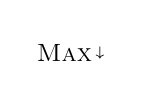
\begin{tikzpicture}[xscale=0.6,yscale=0.4]
\node (max) at (0,0) {{\small \textsc{Max}}};
\node (reg) at (0.75,0.5) {{\fns \textalpha}};
\node (arrow) at (0.75,0) {{\tiny $\downarrow$}};
\node (Rt) at (0.75,-0.5) {{\fns \textbeta}};
\end{tikzpicture}
\end{minipage}
}

\newcommand{\DepAB}{
\begin{minipage}{0.09\textwidth}
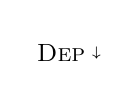
\begin{tikzpicture}[xscale=0.6,yscale=0.4]
\node (max) at (0,0) {{\small \textsc{Dep}}};
\node (reg) at (0.75,0.5) {{\fns \textalpha}};
\node (arrow) at (0.75,0) {{\tiny $\downarrow$}};
\node (Rt) at (0.75,-0.5) {{\fns \textbeta}};
\end{tikzpicture}
\end{minipage}
}

\newcommand{\DepHReg}{
\begin{minipage}{0.055\textwidth}
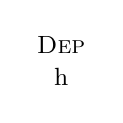
\begin{tikzpicture}[xscale=0.6,yscale=0.4]
\node (dep) at (0,0) {{\small \textsc{Dep}}};
\node (reg) at (0,-1.0) {{\small h}};
\end{tikzpicture}
\end{minipage}
}

\newcommand{\DepLReg}{
\begin{minipage}{0.055\textwidth}
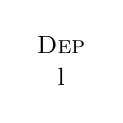
\begin{tikzpicture}[xscale=0.6,yscale=0.4]
\node (dep) at (0,0) {{\small \textsc{Dep}}};
\node (reg) at (0,-1.0) {{\small l}};
\end{tikzpicture}
\end{minipage}
}

\newcommand{\DepReg}{
\begin{minipage}{0.055\textwidth}
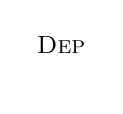
\begin{tikzpicture}[xscale=0.6,yscale=0.4]
\node (dep) at (0,0) {{\small \textsc{Dep}}};
\node (reg) at (0,-1.0) {{\small \textrho}};
\end{tikzpicture}
\end{minipage}
}

\newcommand{\DepTRt}{
\begin{minipage}{0.1\textwidth}
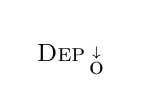
\begin{tikzpicture}[xscale=0.6,yscale=0.4]
\node (dep) at (0,0) {{\small \textsc{Dep}}};
\node (t) at (0.75,0.5) {{\fns \texttau}};
\node (arrow) at (0.75,0) {{\tiny $\downarrow$}};
\node (Rt) at (0.75,-0.5) {{\fns o}};
\end{tikzpicture}
\end{minipage}
}

\newcommand{\MaxRegRt}{
\begin{minipage}{0.1\textwidth}
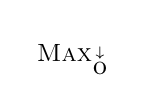
\begin{tikzpicture}[xscale=0.6,yscale=0.4]
\node (max) at (0,0) {{\small \textsc{Max}}};
\node (arrow) at (0.75,0) {{\tiny $\downarrow$}};
\node (Rt) at (0.75,-0.5) {{\fns o}};
\node (reg) at (0.75,0.5) {{\fns \textrho}};
\end{tikzpicture}
\end{minipage}
}

\newcommand{\RegToneByRt}{
\begin{minipage}{0.06\textwidth}
\begin{tikzpicture}[xscale=0.6,yscale=0.5]
\node[rotate=20] (arrow1) at (-0.15,0) {{\fns $\uparrow$}};
\node[rotate=340] (arrow2) at (0.15,0) {{\fns $\uparrow$}};
\node (Rt) at (0,-0.55) {{\small o}};
\node (reg) at (0.4,0.55) {{\small \textrho}};
\node (tone) at (-0.4,0.55) {{\small \texttau}};
\end{tikzpicture}
\end{minipage}
}

\newcommand{\RegToneBySyl}{
\begin{minipage}{0.06\textwidth}
\begin{tikzpicture}[xscale=0.6,yscale=0.5]
\node[rotate=20] (arrow1) at (-0.15,0) {{\fns $\uparrow$}};
\node[rotate=340] (arrow2) at (0.15,0) {{\fns $\uparrow$}};
\node (Rt) at (0,-0.55) {{\small \textsigma}};
\node (reg) at (0.4,0.55) {{\small \textrho}};
\node (tone) at (-0.4,0.55) {{\small \texttau}};
\end{tikzpicture}
\end{minipage}
}

\newcommand{\DepTone}{
\begin{minipage}{0.055\textwidth}
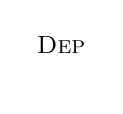
\begin{tikzpicture}[xscale=0.6,yscale=0.4]
\node (dep) at (0,0) {{\small \textsc{Dep}}};
\node (tone) at (0,-1.0) {{\small \texttau}};
\end{tikzpicture}
\end{minipage}
}

\newcommand{\DepTonalRt}{
\begin{minipage}{0.055\textwidth}
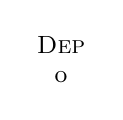
\begin{tikzpicture}[xscale=0.6,yscale=0.4]
\node (dep) at (0,0) {{\small \textsc{Dep}}};
\node (tone) at (0,-1.0) {{\small o}};
\end{tikzpicture}
\end{minipage}
}

\newcommand{\DepL}{
\begin{minipage}{0.055\textwidth}
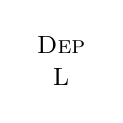
\begin{tikzpicture}[xscale=0.6,yscale=0.4]
\node (dep) at (0,0) {{\small \textsc{Dep}}};
\node (tone) at (0,-1.0) {{\small L}};
\end{tikzpicture}
\end{minipage}
}

\newcommand{\DepH}{
\begin{minipage}{0.055\textwidth}
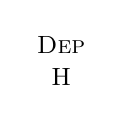
\begin{tikzpicture}[xscale=0.6,yscale=0.4]
\node (dep) at (0,0) {{\small \textsc{Dep}}};
\node (tone) at (0,-1.0) {{\small H}};
\end{tikzpicture}
\end{minipage}
}

\newcommand{\NoMultDiff}{{\small *loh}}
\newcommand{\Alt}{{\small \textsc{Alt}}}
\newcommand{\NoSkip}{{\small \scell{\textsc{No}\\\textsc{Skip}}}}


\newcommand{\RegDomRt}{
\begin{minipage}{0.030\textwidth}
\begin{tikzpicture}[xscale=0.6,yscale=0.5]
\node (arrow) at (0,0) {{\fns $\downarrow$}};
\node (Rt) at (0,-0.55) {{\small o}};
\node (reg) at (0,0.55) {{\small \textrho}};
\end{tikzpicture}
\end{minipage}
}

\newcommand{\DepRegRt}{
\begin{minipage}{0.1\textwidth}
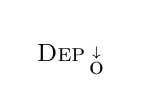
\begin{tikzpicture}[xscale=0.6,yscale=0.4]
\node (dep) at (0,0) {{\small \textsc{Dep}}};
\node (arrow) at (0.75,0) {{\tiny $\downarrow$}};
\node (Rt) at (0.75,-0.5) {{\fns o}};
\node (reg) at (0.75,0.5) {{\fns \textrho}};
\end{tikzpicture}
\end{minipage}
}

% unused

\newcommand{\ToneByRt}{
\begin{minipage}{0.05\textwidth}
\begin{tikzpicture}[xscale=0.6,yscale=0.5]
\node (arrow) at (0,0) {{\fns $\uparrow$}};
\node (Rt) at (0,-0.55) {{\small o}};
\node (tone) at (0,0.55) {{\small \texttau}};
\end{tikzpicture}
\end{minipage}
}

\newcommand{\RegByRt}{
\begin{minipage}{0.05\textwidth}
\begin{tikzpicture}[xscale=0.6,yscale=0.5]
\node (arrow) at (0,0) {{\fns $\uparrow$}};
\node (Rt) at (0,-0.55) {{\small o}};
\node (reg) at (0,0.55) {{\small \textrho}};
\end{tikzpicture}
\end{minipage}
}

\newcommand{\ToneDomRt}{
\begin{minipage}{0.05\textwidth}
\begin{tikzpicture}[xscale=0.6,yscale=0.5]
\node (arrow) at (0,0) {{\fns $\downarrow$}};
\node (Rt) at (0,-0.55) {{\small o}};
\node (tone) at (0,0.55) {{\small \texttau}};
\end{tikzpicture}
\end{minipage}
}

% --- OT tableaus --- %

% Sec. 3.2, first tabl.

\newcommand{\OTHLInput}{
\begin{minipage}{0.17\textwidth}
\begin{tikzpicture}[xscale=\myscalex,yscale=\myscaley]
\node (tone) at (2,0) {(= H)};
\node (syl) at (0,0) {\textsigma};
\node (Rt) at (0,1) {o};
\node (H) at (-0.5,2) {H};
\node (R) at (0.5,3) {h};
\node (Rt2) at (1.5,1.0) {o};
%\node (H2) at (1.0,2) {\epen{L}};
\node (R2) at (2.0,3) {\blue{l}};
\draw [thick] (syl.north) -- (Rt.south) ;
\draw [thick] (Rt.north) -- (H.south) ;
\draw [thick] (Rt.north) -- (R.south) ;
\draw [thick] (syl.north) -- (Rt2.south) ;
%\draw [dashed] (Rt2.north) -- (H2.south) ;
%\draw [dashed] (Rt2.north) -- (R2.south) ;
\end{tikzpicture}
\end{minipage}
}

\newcommand{\OTHLWinner}{
\begin{minipage}{0.17\textwidth}
\begin{tikzpicture}[xscale=\myscalex,yscale=\myscaley]
\node (tone) at (2,0) {(= HL)};
\node (syl) at (0,0) {\textsigma};
\node (Rt) at (0,1) {o};
\node (H) at (-0.5,2) {H};
\node (R) at (0.5,3) {h};
\node (Rt2) at (1.5,1.0) {o};
\node (H2) at (1.0,2) {\epen{L}};
\node (R2) at (2.0,3) {\blue{l}};
\draw [thick] (syl.north) -- (Rt.south) ;
\draw [thick] (Rt.north) -- (H.south) ;
\draw [thick] (Rt.north) -- (R.south) ;
\draw [thick] (syl.north) -- (Rt2.south) ;
\draw [dashed] (Rt2.north) -- (H2.south) ;
\draw [dashed] (Rt2.north) -- (R2.south) ;
\end{tikzpicture}
\end{minipage}
}

\newcommand{\OTHLSpreadingHOnly}{
\begin{minipage}{0.17\textwidth}
\begin{tikzpicture}[xscale=\myscalex,yscale=\myscaley]
\node (tone) at (2,0) {(= HM)};
\node (syl) at (0,0) {\textsigma};
\node (Rt) at (0,1) {o};
\node (H) at (-0.5,2) {H};
\node (R) at (0.5,3) {h};
\node (Rt2) at (1.5,1.0) {o};
%\node (H2) at (1.0,2) {\epen{L}};
\node (R2) at (2.0,3) {\blue{l}};
\draw [thick] (syl.north) -- (Rt.south) ;
\draw [thick] (Rt.north) -- (H.south) ;
\draw [thick] (Rt.north) -- (R.south) ;
\draw [thick] (syl.north) -- (Rt2.south) ;
\draw [dashed] (Rt2.north) -- (R2.south) ;
\draw [dashed] (Rt2.north) -- (H.south) ;
\end{tikzpicture}
\end{minipage}
}

\newcommand{\OTHLInsertH}{
\begin{minipage}{0.17\textwidth}
\begin{tikzpicture}[xscale=\myscalex,yscale=\myscaley]
\node (tone) at (2,0) {(= HM)};
\node (syl) at (0,0) {\textsigma};
\node (Rt) at (0,1) {o};
\node (H) at (-0.5,2) {H};
\node (R) at (0.5,3) {h};
\node (Rt2) at (1.5,1.0) {o};
\node (H2) at (1.0,2) {\epen{H}};
\node (R2) at (2.0,3) {\blue{l}};
\draw [thick] (syl.north) -- (Rt.south) ;
\draw [thick] (Rt.north) -- (H.south) ;
\draw [thick] (Rt.north) -- (R.south) ;
\draw [thick] (syl.north) -- (Rt2.south) ;
\draw [dashed] (Rt2.north) -- (H2.south) ;
\draw [dashed] (Rt2.north) -- (R2.south) ;
\end{tikzpicture}
\end{minipage}
}

\newcommand{\OTHLOverwriting}{
\begin{minipage}{0.17\textwidth}
\begin{tikzpicture}[xscale=\myscalex,yscale=\myscaley]
\node (syl) at (0,0) {\textsigma};
\node (Rt) at (0,1) {o};
\node (H) at (-0.5,2) {H};
\node (R) at (0.5,3) {h};
\node (Rt2) at (1.5,1.0) {o};
%\node (H2) at (1.0,2) {\epen{L}};
\node (R2) at (2.0,3) {\blue{l}};
\draw [thick] (syl.north) -- (Rt.south) ;
\draw [thick] (Rt.north) -- (H.south) ;
\draw [thick] (Rt.north) -- (R.south) ;
\draw [thick] (syl.north) -- (Rt2.south) ;
%\draw [dashed] (Rt2.north) -- (H2.south) ;
\draw [dashed] (Rt.north) -- (R2.south) ;
\node (del) at (0.3,1.9) {\textbf{=}};
\end{tikzpicture}
\end{minipage}
}

\newcommand{\OTHLSpreading}{
\begin{minipage}{0.17\textwidth}
\begin{tikzpicture}[xscale=\myscalex,yscale=\myscaley]
\node (syl) at (0,0) {\textsigma};
\node (Rt) at (0,1) {o};
\node (H) at (-0.5,2) {H};
\node (R) at (0.5,3) {h};
\node (Rt2) at (1.5,1.0) {o};
%\node (H2) at (1.0,2) {\epen{L}};
\node (R2) at (2.0,3) {\blue{l}};
\draw [thick] (syl.north) -- (Rt.south) ;
\draw [thick] (Rt.north) -- (H.south) ;
\draw [thick] (Rt.north) -- (R.south) ;
\draw [thick] (syl.north) -- (Rt2.south) ;
%\draw [dashed] (Rt2.north) -- (H2.south) ;
\draw [dashed] (Rt2.north) -- (H.south) ;
\draw [dashed] (Rt2.north) -- (R.south) ;
\end{tikzpicture}
\end{minipage}
}

% Sec. 4.2, second tabl.: phrase-medial position

\newcommand{\OTHnoLInput}{
\begin{minipage}{0.17\textwidth}
\begin{tikzpicture}[xscale=\myscalex,yscale=\myscaley]
\node (tone) at (2,0) {(= H)};
\node (syl) at (0,0) {\textsigma};
\node (Rt) at (0,1) {o};
\node (H) at (-0.5,2) {H};
\node (R) at (0.5,3) {h};
\node (Rt2) at (1.5,1.0) {o};
%\node (H2) at (1.0,2) {\epen{L}};
%\node (R2) at (2.0,3) {\blue{l}};
\draw [thick] (syl.north) -- (Rt.south) ;
\draw [thick] (Rt.north) -- (H.south) ;
\draw [thick] (Rt.north) -- (R.south) ;
\draw [thick] (syl.north) -- (Rt2.south) ;
\end{tikzpicture}
\end{minipage}
}

\newcommand{\OTHnoLEpenth}{
\begin{minipage}{0.17\textwidth}
\begin{tikzpicture}[xscale=\myscalex,yscale=\myscaley]
\node (tone) at (2,0) {(= HM)};
\node (syl) at (0,0) {\textsigma};
\node (Rt) at (0,1) {o};
\node (H) at (-0.5,2) {H};
\node (R) at (0.5,3) {h};
\node (Rt2) at (1.5,1.0) {o};
\node (H2) at (1.0,2) {\epen{L}};
\node (R2) at (2.0,3) {\epen{h}};
\draw [thick] (syl.north) -- (Rt.south) ;
\draw [thick] (Rt.north) -- (H.south) ;
\draw [thick] (Rt.north) -- (R.south) ;
\draw [thick] (syl.north) -- (Rt2.south) ;
\draw [dashed] (Rt2.north) -- (H2.south) ;
\draw [dashed] (Rt2.north) -- (R2.south) ;
\end{tikzpicture}
\end{minipage}
}

\newcommand{\OTHnoLSpreading}{
\begin{minipage}{0.17\textwidth}
\begin{tikzpicture}[xscale=\myscalex,yscale=\myscaley]
\node (tone) at (2,0) {(= HH)};
\node (syl) at (0,0) {\textsigma};
\node (Rt) at (0,1) {o};
\node (H) at (-0.5,2) {H};
\node (R) at (0.5,3) {h};
\node (Rt2) at (1.5,1.0) {o};
%\node (H2) at (1.0,2) {\epen{L}};
%\node (R2) at (2.0,3) {\blue{l}};
\draw [thick] (syl.north) -- (Rt.south) ;
\draw [thick] (Rt.north) -- (H.south) ;
\draw [thick] (Rt.north) -- (R.south) ;
\draw [thick] (syl.north) -- (Rt2.south) ;
\draw [dashed] (Rt2.north) -- (H.south) ;
\draw [dashed] (Rt2.north) -- (R.south) ;
\end{tikzpicture}
\end{minipage}
}

% Sec. 4.2, third tabl., LM is unaffected by L\%

\newcommand{\OTLMInput}{
\begin{minipage}{0.2\textwidth}
\begin{tikzpicture}[xscale=\myscalex,yscale=\myscaley]
\node (tone) at (2,0) {(= LM)};
\node (syl) at (0,0) {\textsigma};
\node (Rt) at (0,1) {o};
\node (H) at (-0.5,2) {L};
\node (R) at (0.5,3) {l};
\node (Rt2) at (1.5,1.0) {o};
\node (H2) at (1.0,2) {L};
\node (R2) at (2.0,3) {h};
\node (R3) at (3.0,3) {\blue{l}};
\draw [thick] (syl.north) -- (Rt.south) ;
\draw [thick] (Rt.north) -- (H.south) ;
\draw [thick] (Rt.north) -- (R.south) ;
\draw [thick] (syl.north) -- (Rt2.south) ;
\draw [thick] (Rt2.north) -- (H2.south) ;
\draw [thick] (Rt2.north) -- (R2.south) ;
\end{tikzpicture}
\end{minipage}
}

\newcommand{\OTLMReplace}{
\begin{minipage}{0.2\textwidth}
\begin{tikzpicture}[xscale=\myscalex,yscale=\myscaley]
\node (tone) at (2,0) {(= LL)};
\node (syl) at (0,0) {\textsigma};
\node (Rt) at (0,1) {o};
\node (H) at (-0.5,2) {L};
\node (R) at (0.5,3) {l};
\node (Rt2) at (1.5,1.0) {o};
\node (H2) at (1.0,2) {L};
\node (R2) at (2.0,3) {h};
\node (R3) at (3.0,3) {\blue{l}};
\draw [thick] (syl.north) -- (Rt.south) ;
\draw [thick] (Rt.north) -- (H.south) ;
\draw [thick] (Rt.north) -- (R.south) ;
\draw [thick] (syl.north) -- (Rt2.south) ;
\draw [thick] (Rt2.north) -- (H2.south) ;
\draw [thick] (Rt2.north) -- (R2.south) ;
\draw [dashed] (Rt2.north) -- (R3.south) ;
\node (del) at (1.8,2.1) {\textbf{=}};
\end{tikzpicture}
\end{minipage}
}

\newcommand{\OTLMTwoReg}{
\begin{minipage}{0.2\textwidth}
\begin{tikzpicture}[xscale=\myscalex,yscale=\myscaley]
\node (tone) at (2,0) {(= LML)};
\node (syl) at (0,0) {\textsigma};
\node (Rt) at (0,1) {o};
\node (H) at (-0.5,2) {L};
\node (R) at (0.5,3) {l};
\node (Rt2) at (1.5,1.0) {o};
\node (H2) at (1.0,2) {L};
\node (R2) at (2.0,3) {h};
\node (R3) at (3.0,3) {\blue{l}};
\draw [thick] (syl.north) -- (Rt.south) ;
\draw [thick] (Rt.north) -- (H.south) ;
\draw [thick] (Rt.north) -- (R.south) ;
\draw [thick] (syl.north) -- (Rt2.south) ;
\draw [thick] (Rt2.north) -- (H2.south) ;
\draw [thick] (Rt2.north) -- (R2.south) ;
\draw [dashed] (Rt2.north) -- (R3.south) ;
\end{tikzpicture}
\end{minipage}
}

% Sec. 4.2, fourth tabl., L is affected by L\% but M is not

\newcommand{\OTLInput}{
\begin{minipage}{0.17\textwidth}
\begin{tikzpicture}[xscale=\myscalex,yscale=\myscaley]
\node (tone) at (2,0) {(= L)};
\node (syl) at (0,0) {\textsigma};
\node (Rt) at (0,1) {o};
\node (H) at (-0.5,2) {L};
\node (R) at (0.5,3) {l};
\node (R2) at (2,3) {\blue{l}};
\draw [thick] (syl.north) -- (Rt.south) ;
\draw [thick] (Rt.north) -- (H.south) ;
\draw [thick] (Rt.north) -- (R.south) ;
\end{tikzpicture}
\end{minipage}
}

\newcommand{\OTLLowered}{
\begin{minipage}{0.17\textwidth}
\begin{tikzpicture}[xscale=\myscalex,yscale=\myscaley]
\node (tone) at (2,0) {(= LL)};
\node (syl) at (0,0) {\textsigma};
\node (Rt) at (0,1) {o};
\node (H) at (-0.5,2) {L};
\node (R) at (0.5,3) {l};
\node (R2) at (2,3) {\blue{l}};
\draw [thick] (syl.north) -- (Rt.south) ;
\draw [thick] (Rt.north) -- (H.south) ;
\draw [thick] (Rt.north) -- (R.south) ;
\draw [dashed] (Rt.north) -- (R2.south) ;
\end{tikzpicture}
\end{minipage}
}

\newcommand{\OTMInput}{
\begin{minipage}{0.17\textwidth}
\begin{tikzpicture}[xscale=\myscalex,yscale=\myscaley]
\node (tone) at (2,0) {(= M)};
\node (syl) at (0,0) {\textsigma};
\node (Rt) at (0,1) {o};
\node (H) at (-0.5,2) {L};
\node (R) at (0.5,3) {h};
\node (R2) at (2,3) {\blue{l}};
\draw [thick] (syl.north) -- (Rt.south) ;
\draw [thick] (Rt.north) -- (H.south) ;
\draw [thick] (Rt.north) -- (R.south) ;
\end{tikzpicture}
\end{minipage}
}

\newcommand{\OTMLowered}{
\begin{minipage}{0.17\textwidth}
\begin{tikzpicture}[xscale=\myscalex,yscale=\myscaley]
\node (tone) at (2,0) {(= ML)};
\node (syl) at (0,0) {\textsigma};
\node (Rt) at (0,1) {o};
\node (H) at (-0.5,2) {L};
\node (R) at (0.5,3) {h};
\node (R2) at (2,3) {\blue{l}};
\draw [thick] (syl.north) -- (Rt.south) ;
\draw [thick] (Rt.north) -- (H.south) ;
\draw [thick] (Rt.north) -- (R.south) ;
\draw [dashed] (Rt.north) -- (R2.south) ;
\end{tikzpicture}
\end{minipage}
}

% Sec. 4.2, fifth tableau, polar questions with level tones

\newcommand{\OTLPolIn}{
\begin{minipage}{0.20\textwidth}
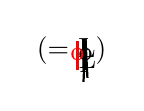
\begin{tikzpicture}[xscale=\myscalex-0.05,yscale=\myscaley-0.05]
\node (tone) at (3.5,0) {(= L)};
\node (syl) at (0,0) {\textsigma};
\node (syl2) at (2,0) {\red{\textsigma}};
\node (Rt) at (0,1) {o};
\node (H) at (-0.5,2) {L};
\node (R) at (0.5,3) {l};
\node (Rt2) at (2,1) {\red{o}};
\draw [thick] (syl.north) -- (Rt.south) ;
\draw [thick,red] (syl2.north) -- (Rt2.south) ;
\draw [thick] (Rt.north) -- (H.south) ;
\draw [thick] (Rt.north) -- (R.south) ;
\end{tikzpicture}
\end{minipage}
}

\newcommand{\OTLPolDef}{
\begin{minipage}{0.20\textwidth}
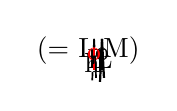
\begin{tikzpicture}[xscale=\myscalex-0.05,yscale=\myscaley-0.05]
\node (tone) at (3.5,0) {(= L.M)};
\node (syl) at (0,0) {\textsigma};
\node (syl2) at (2,0) {\red{\textsigma}};
\node (Rt) at (0,1) {o};
\node (H) at (-0.5,2) {L};
\node (R) at (0.5,3) {l};
\node (H2) at (1.5,2) {\epen{L}};
\node (R2) at (2.5,3) {\epen{h}};
\node (Rt2) at (2,1) {\red{o}};
\draw [thick] (syl.north) -- (Rt.south) ;
\draw [thick,red] (syl2.north) -- (Rt2.south) ;
\draw [thick] (Rt.north) -- (H.south) ;
\draw [thick] (Rt.north) -- (R.south) ;
\draw [semithick,dashed] (Rt2.north) -- (H2.south) ;
\draw [semithick,dashed] (Rt2.north) -- (R2.south) ;
\end{tikzpicture}
\end{minipage}
}

\newcommand{\OTLPolAlt}{
\begin{minipage}{0.20\textwidth}
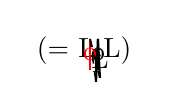
\begin{tikzpicture}[xscale=\myscalex-0.05,yscale=\myscaley-0.05]
\node (tone) at (3.5,0) {(= L.L)};
\node (syl) at (0,0) {\textsigma};
\node (syl2) at (2,0) {\red{\textsigma}};
\node (Rt) at (0,1) {o};
\node (H) at (-0.5,2) {L};
\node (R) at (0.5,3) {l};
\node (Rt2) at (2,1) {\red{o}};
\draw [thick] (syl.north) -- (Rt.south) ;
\draw [thick,red] (syl2.north) -- (Rt2.south) ;
\draw [thick] (Rt.north) -- (H.south) ;
\draw [thick] (Rt.north) -- (R.south) ;
\draw [semithick,dashed] (Rt2.north) -- (H.south) ;
\draw [semithick,dashed] (Rt2.north) -- (R.south) ;
\end{tikzpicture}
\end{minipage}
}

% Sec. 4.2, sixth tableau, polar questions with contour tones

\newcommand{\OTLLPolIn}{
\begin{minipage}{0.23\textwidth}
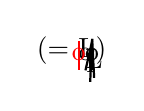
\begin{tikzpicture}[xscale=\myscalex-0.05,yscale=\myscaley-0.05]
\node (tone) at (5.2,0) {(= L)};
\node (syl) at (0,0) {\textsigma};
\node (syl3) at (3.4,0) {\red{\textsigma}};
\node (Rt) at (0,1) {o};
\node (Rt2) at (1.7,1) {o};
\node (Rt3) at (3.4,1) {\red{o}};
\node (H) at (-0.5,2) {L};
\node (R) at (0.5,3) {l};
\draw [thick] (syl.north) -- (Rt.south) ;
\draw [thick] (syl.north) -- (Rt2.south) ;
\draw [thick,red] (syl3.north) -- (Rt3.south) ;
\draw [thick] (Rt.north) -- (H.south) ;
\draw [thick] (Rt.north) -- (R.south) ;
\end{tikzpicture}
\end{minipage}
}

\newcommand{\OTLLPolDef}{
\begin{minipage}{0.23\textwidth}
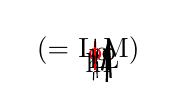
\begin{tikzpicture}[xscale=\myscalex-0.05,yscale=\myscaley-0.05]
\node (tone) at (5.2,0) {(= L.M)};
\node (syl) at (0,0) {\textsigma};
\node (syl3) at (3.4,0) {\red{\textsigma}};
\node (Rt) at (0,1) {o};
\node (Rt2) at (1.7,1) {o};
\node (Rt3) at (3.4,1) {\red{o}};
\node (H) at (-0.5,2) {L};
\node (R) at (0.5,3) {l};
\node (H3) at (2.9,2) {\epen{L}};
\node (R3) at (3.9,3) {\epen{h}};
\draw [thick] (syl.north) -- (Rt.south) ;
\draw [thick] (syl.north) -- (Rt2.south) ;
\draw [thick,red] (syl3.north) -- (Rt3.south) ;
\draw [thick] (Rt.north) -- (H.south) ;
\draw [thick] (Rt.north) -- (R.south) ;
\draw [dashed] (Rt3.north) -- (H3.south) ;
\draw [dashed] (Rt3.north) -- (R3.south) ;
\end{tikzpicture}
\end{minipage}
}

\newcommand{\OTLLPolSkip}{
\begin{minipage}{0.23\textwidth}
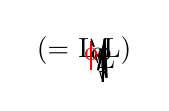
\begin{tikzpicture}[xscale=\myscalex-0.05,yscale=\myscaley-0.05]
\node (tone) at (5.2,0) {(= L.L)};
\node (syl) at (0,0) {\textsigma};
\node (syl3) at (3.4,0) {\red{\textsigma}};
\node (Rt) at (0,1) {o};
\node (Rt2) at (1.7,1) {o};
\node (Rt3) at (3.4,1) {\red{o}};
\node (H) at (-0.5,2) {L};
\node (R) at (0.5,3) {l};
\draw [thick] (syl.north) -- (Rt.south) ;
\draw [thick] (syl.north) -- (Rt2.south) ;
\draw [thick,red] (syl3.north) -- (Rt3.south) ;
\draw [thick] (Rt.north) -- (H.south) ;
\draw [thick] (Rt.north) -- (R.south) ;
\draw [dashed] (Rt3.north) -- (H.south) ;
\draw [dashed] (Rt3.north) -- (R.south) ;
\end{tikzpicture}
\end{minipage}
}  
  
\newcommand{\ilit}[1]{#1\il{#1}}    
\newcommand{\isit}[1]{#1\is{#1}}  

\makeatletter
\let\thetitle\@title
\let\theauthor\@author 
\makeatother

\newcommand{\togglepaper}[1][0]{ 
  \bibliography{../localbibliography}
  %% hyphenation points for line breaks
%% Normally, automatic hyphenation in LaTeX is very good
%% If a word is mis-hyphenated, add it to this file
%%
%% add information to TeX file before \begin{document} with:
%% %% hyphenation points for line breaks
%% Normally, automatic hyphenation in LaTeX is very good
%% If a word is mis-hyphenated, add it to this file
%%
%% add information to TeX file before \begin{document} with:
%% \include{localhyphenation}
\hyphenation{
affri-ca-te
affri-ca-tes
com-ple-ments
par-a-digm
Sha-ron
Kings-ton
phe-nom-e-non
Daul-ton
Abu-ba-ka-ri
Ngo-nya-ni
Clem-ents 
King-ston
Tru-cken-brodt
Tab-leau
cophono-logies
mark-edness
Ti-gri-nya
a-mong
Car-stens
Lu-bu-ku-su
}
\hyphenation{
affri-ca-te
affri-ca-tes
com-ple-ments
par-a-digm
Sha-ron
Kings-ton
phe-nom-e-non
Daul-ton
Abu-ba-ka-ri
Ngo-nya-ni
Clem-ents 
King-ston
Tru-cken-brodt
Tab-leau
cophono-logies
mark-edness
Ti-gri-nya
a-mong
Car-stens
Lu-bu-ku-su
}
  \papernote{\scriptsize\normalfont
    \theauthor.
    \thetitle. 
    To appear in: 
    Emily Clem,   Peter Jenks \& Hannah Sande.
    Theory and description in African Linguistics: Selected papers from the 47th Annual Conference on African Linguistics.
    Berlin: Language Science Press. [preliminary page numbering]
  }
  \pagenumbering{roman}
  \setcounter{chapter}{#1}
  \addtocounter{chapter}{-1}
}

\newcommand{\upstep}{\textupstep}


% \newcounter{tableauxcounter}

\renewcommand{\textltailn}{ɲ}
\renewcommand{\textbardotlessj}{ɟ}

\newcommand{\emphkh}[1]{\textit{#1}} %originally \textbf, banned by the guidelines



\definecolor{lsDOIGray}{cmyk}{0,0,0,0.45}


\newcommand{\xuparrow}[1]{%
  {\left\uparrow\vbox to #1{}\right.\kern-\nulldelimiterspace}
}
\renewcommand \textupstep[1]{\char"A71B#1}
\renewcommand \textdownstep[1]{\char"A71C#1}
 
 \newcommand{\ꜛ}{\textsf{ꜛ}}
 
\def\biberror{\undefined}


\newcommand{\OTbox}[1]{\resizebox{.88\textwidth}{!}{#1}}
 

\author{Ọbádélé Bakari Kambon\affiliation{University of Ghana, Legon}\and Reginald Akuoko Duah\affiliation{University of Ghana, Legon}\lastand Clement Kwamina Insaidoo Appah\affiliation{University of Ghana, Legon}}
\title{Serial verb nominalization in Akan: The question of intervening elements}

\abstract{In this paper, we hope to disambiguate the nature of look-alike intervening elements that appear between verbs in Serial Verb Constructions (SVCs) and Serial Verb Construction Nominalizations (SVCNs). To do so, we will first show that these intervening elements share the same phonological form. We will then show that although the intervening elements look the same on the surface, they can be differentiated by appealing to semantics and the construction from which the SVCN is derived. In doing so, we find that some of the intervening elements should, indeed, be regarded as \textsc{tamp} markers, while others are nominalizers (\textsc{nmlz}). In conclusion, we identify abstract schemata/templates that account for, and predict the positioning of, intervening elements found in Akan SVCNs. 
}

\begin{document}

\graphicspath{{figures/}}

\maketitle

\section{Background}\label{sec:duah:1}
In this paper, we address the question of intervening elements in nominalized Serial Verb Constructions (SVCs).\footnote{This project originated from a question from Clement Appah at the PhD defense of Ọbádélé Bakari Kambon in which it was asked how do we know that the intervening elements between nominalized verbs from Serial Verb Constructions (SVCs) are actually tense, \isi{aspect}, mood, polarity (\textsc{tamp}) markers and not simply nominal markers. The video of the PhD defense can be viewed here: \url{https://youtu.be/QXDFwLV0Atc}.}  Tense, \isi{aspect}, mood and polarity (\textsc{tamp}) markers surface with the same \isi{phonological form} as nominalizing affixes (\textsc{nmlz}) in \ili{Akan}. We hope to show, with evidence, times in which such intervening elements are grammatical elements derived from the original \isi{serial verb} construction -- such as \textsc{tamp} markers, etc. -- and when they are actually nominal elements (\textsc{nmlz}). To do so, we will first substantiate that nominalized verbs in \ili{Akan} are made with /a-/ and /-N-/, which are the same affixes that can be found as \textsc{tamp} markers in SVCs. While this identity of form could potentially lead to ambiguity in terms of analysis, there are some clear cues in terms of form, function and semantics that can help us to disambiguate and clearly identify intervening elements. What makes the investigation special with regard to SVCs relates to the intervening element available, depending on what type of SVC instantiated. In SVCs, the intervening elements may be either \textsc{nmlz} or \textsc{tamp}. We do not, however, find \textsc{tamp} markers on single verbs; only nominalizers. The observation that \textsc{tamp} can occur in the case of SVCs makes this investigation intriguing and it brings out a phenomenon that could not be observed if we were dealing with single verbs alone. 
 
Pioneering work on SVC nominalization has been done in the last few decades \citep{bodomo1994,bodomo2004,bodomo2006,hiraiwabodomo2008,aboh2009,kambon2012}. Following \citet{bodomo1994}, much of this literature has followed the terminology of ``Serial Verb Nominalization.'' However, given that other constituents, when they appear in the SVC, also must surface in the nominal form, we prefer the term Serial Verb Construction Nominalization (SVCN). We feel that this terminology better accounts for all constituents of the construction and its nominalized form, whether or not these elements happen to be verbs or not.\footnote{See \citet{kambon2012} and \citet{kambon2015} for a discussion on revising some criteria and definitions of SVCs.}    
 
There are several potential ways of categorizing or typologizing SVCs. Such ways include on the basis of transitivity of included verbs, whether or not argument sharing exists, and/or based on the degree of idiomaticity, semantic integration and lexicalization. Following \citet{osam1994} categorization of SVCs based on degree of semantic integration (and associated degrees of lexicalization) \citet{kambon2012} showed that there are progressively greater degrees of integration ranging from the non-integrated Chaining Serial Constructions (CSCs) to Partial Lexicalized-Integrated Serial Verb Constructions (PL-ISVCs) to the most integrated Full Lexicalized-Integrated Serial Verb Constructions (FL-ISVCs).
 
 \pagebreak
The relationship between Semantic Integration and Lexicalization can be captured in \figref{fig:duah:1}, which shows that as there is less conceptual distance between events, this is manifested in terms of progressively more lexicalization as expressed in the language.\\
 
\begin{figure} 

Separate sentences $\rightarrow$ Coordination $\rightarrow$ CSC $\rightarrow$ PL-ISVC $\rightarrow$ FL-ISVC $\rightarrow$ Single Verb

\caption{\label{fig:duah:1}Scale of lessening conceptual distance \citep[95]{kambon2012}}
\end{figure}

Using Semantic Integration and Lexicalization as a means of categorization, \citet{kambon2012} showed that 98.63\% (144 out of 146) of all FL-ISVCs identified have nominal counterparts while only 2.46\% (17 out of 690) of all PL-ISVCs identified have nominal counterparts. CSCs, on the other hand seem to nominalize haphazardly as designata and denotata in the form of apparently random frozen proverbs, idioms/figures of speech and sentences.

While it is not our intention to rehash the entire means for identifying the FL-ISVCs to distinguish them from PL-ISVCs, it was decided that an independent means (other than nominalization itself, which would lead to circular argumentation) should be employed in order to categorize each one. Part of this came from \posscitet{osam1994} initial discussion of FL-ISVCs, in which he writes, ``Ranking high on the scale of integration are those verbal combinations that have become {fully lexicalised into verb compounds} and which are used as {\textit{lexicalised idioms}}.'' \citep[238, emphasis added]{osam1994}. In recognizing that there was a link between semantic integration and idiomaticity, we employed \posscitet{barkema1996} schema, which deals with defining characteristics of idioms on the basis of collocability, familiarity, flexibility and compositionality to test the idiomaticity and/or semantic integration of different types of SVCs identified for \ili{Akan}. \textbf{Flexibility} deals with the degree to which a given idiom may take on various grammatical forms (i.e. number, specification, other types of morphological marking) without ``breaking'' the idiom and forcing a literal interpretation. \textsc{Compositionality} can be understood as the ``degree to which the sum total meaning of the entire construction is readily derived from the parts contained therein'' \citet[47]{kambon2012}. \textsc{Collocability} may be thought of as the ``degree to which synonym or antonym alternatives can be freely switched in and out'' \citet[46]{kambon2012}. \textsc{Familiarity} involves the currency of the idiom whereby it has become institutionalized to the point that the idiom, rather than the literal counterfeit form, is assumed by native speakers \citep{kambon2012}. 

Using \posscitet{barkema1996} schema, FL-ISVCs were identified on the basis of the following characteristics:
\begin{itemize}
	\item Usually non-compositional
	\item Usually collocationally closed
	\item Usually inflexible
	\item Usually familiar (institutionalized)
\end{itemize}

In \sectref{sec:duah:3}, we will argue that a key to understanding the nature of intervening elements in SVCNs is identifying the type of SVC source construction from which the SVCN is derived. Below, we illustrate with examples the various types of SVCs and their nominalized counterparts. We begin with examples of FL-ISVCs and nominalized counterparts.\footnote{For consistency of presentation, examples come from \ili{Asante} Twi unless otherwise indicated.}

\ea\label{ex:duah:1}
\ea\label{ex:duah:1a}
\gll Yɛ̀-à-ká yɛ̀n hó á-bɔ̀ mú.\\
1\textsc{pl}-\textsc{prf}-touch 1\textsc{pl.poss} body \textsc{prf}-strike inside\\
\glt `We have united ourselves.'
\ex\label{ex:duah:1b}
\gll Ǹ-ká-bó-m(ú)\\
$^{\text{?}}$\textsc{nmlz}/$^{\text{?}}$\textsc{neg}-touch-strike-inside\\
\glt `Unity'
\ex Ǹkábóḿ hìá yɛ́ń.\\
unity need	1\textsc{pl}\\
\glt `Unity is important to us.'
\z
\z

\ea\label{ex:duah:2}
\ea\label{ex:duah:2a}
\gll Ɔ̀-ǹ-tú nè hó ǹ-kyɛ́.\\
3\textsc{sg}.\textsc{sbj}-\textsc{neg}-uproot	 3\textsc{sg}.\textsc{poss} body \textsc{neg}-give.as.gift\\
\glt `He doesn’t volunteer.'
\ex\label{ex:duah:2b}
\gll À-tù-hó-á-kyɛ́\\
$^{\text{?}}$\textsc{nmlz}/$^{\text{?}}$\textsc{prf}-uproot-body-$^{\text{?}}$\textsc{nmlz}/$^{\text{?}}$\textsc{prf}-give.as.gift\\
\glt `Volunteerism'
\ex \gll Ɔ̀-wɔ̀ àhùmɔ́bórɔ́ né àtùhóákyɛ́.\\
3\textsc{sg}.\textsc{sbj}-possess mercy and volunteerism\\
\glt `He is merciful and has a volunteering spirit.' (lit. he has mercy and volunteerism)
\z
\z

Examples of FL-ISVCs with nominalized counterparts that have potentially ambiguous intervening elements:  

\ea\label{ex:duah:3}
\ea\label{ex:duah:3a}
\gll Mè-ǹ-gyé ásɛ́ḿ nó ń-tò mú.\\
1\textsc{sg}.\textsc{sbj}-\textsc{neg}-receive	word \textsc{det} \textsc{neg}-throw inside\\
\glt `I don’t accept the story.'
\ex\label{ex:duah:3b}
\gll Ǹ-gyé-ń-tó-ḿ(ú)\\
$^{\text{?}}$\textsc{nmlz}/$^{\text{?}}$\textsc{neg}-receive-$^{\text{?}}$\textsc{nmlz}/$^{\text{?}}$\textsc{neg}-throw-inside\\
\glt `Acceptance'
\ex\label{ex:duah:3c}
\gll Ǹnyéńtóḿ(ú) á-m̀-mà só wɔ̀ hɔ́.\\
acceptance \textsc{pst}-\textsc{neg}-come	top	at there\\
\glt `There was no acceptance there (between two or more people).'
\z
\z

\ea\label{ex:duah:4}
\ea\label{ex:duah:4a}
\gll Ɔ̀-à-twá àsɛ́ḿ á-tò mè só.\\
3\textsc{sg}.\textsc{sbj}-\textsc{prf}-cut matter \textsc{prf}-throw 1\textsc{sg}.\textsc{poss} top\\
\glt `He has falsely accused me.'
\ex\label{ex:duah:4b}
\gll Ǹ-twá-ń-tó-só\\
$^{\text{?}}$\textsc{nmlz}/$^{\text{?}}$\textsc{neg}-cut-$^{\text{?}}$\textsc{nmlz}/$^{\text{?}}$\textsc{neg}-throw-top\\
\glt `False accusation'
\ex\label{ex:duah:4c}
\gll Dèɛ̀ 	wó-á-ká yí nyìnáá yɛ̀ ǹtwáńtósó.\\
thing 2\textsc{sg}.\textsc{sbj}-\textsc{prf}-speak \textsc{dem}	all be \isi{false accusation}\\
\glt `All that you are saying is a {false.accusation}.'
\z
\z

A point that will be returned to later that should be noted here is that the prefix /a-/ in (\ref{ex:duah:1}a) and (\ref{ex:duah:4}a) is functioning as a \isi{perfect} marker (\textsc{prf}). Meanwhile /a-/ occurs in the nominalized SVC in (\ref{ex:duah:2}b) and can be analyzed as functioning as a nominalizing prefix (\textsc{nmlz}). Likewise, the prefix /N-/ in (\ref{ex:duah:1}b), (\ref{ex:duah:3}b) and (\ref{ex:duah:4}b) seems to serve as a nominalizing prefix (\textsc{nmlz}), while /N-/ in (\ref{ex:duah:2}a) and (\ref{ex:duah:3}a), a superficially similar /N-/, is \textsc{neg}. Thus, the same phonological forms are serving different functions in the language. The disambiguation of these surface similarities of form is the basis of the primary research agenda of this paper.

PL-ISVCs were also identified as being generally on the other end of the scale as they are:

\begin{itemize}
\item Usually fully compositional
\item Usually collocationally limited
\item Usually semi-flexible (productive)
\item Usually partially familiar (somewhat institutionalized)
\end{itemize}

\ea\label{ex:duah:5}
\ea\label{ex:duah:5a}
\gll Ɔ̀-à-tɔ́ àdùàné á-dì.\\
3\textsc{sg}.\textsc{sbj}-\textsc{prf}-buy food \textsc{prf}-eat\\
\glt `He has bought food to eat.'
\ex\label{ex:duah:5b}
\gll Ǹ-tɔ́-dí-(ɛ́)\\
\textsc{nmlz}-buy-eat-\textsc{nmlz}\\
\glt `Things bought and eaten.'
\ex\label{ex:duah:5c}
\gll Ɔ̀-tàá dí ǹtódíɛ́.\\
3\textsc{sg}.\textsc{sbj}-often	eat	buying-and-eating\\
\glt `He often buys what he eats.'
\z
\z

\ea\label{ex:duah:6}
\ea\label{ex:duah:6a}
\gll Mógyá nà nànánóm hwìè gù-ì.\\
blood \textsc{prt} ancestors pour spill-\textsc{pst}\\
\glt `It is blood that our ancestors shed.'
\ex\label{ex:duah:6b}
\gll Hwìè	-gú-(ó)\\
pour-spill-\textsc{nmlz}\\
\glt `Pouring away'
\ex\label{ex:duah:6c}
\gll Hwìègúó kwà níé.\\
Pouring-away worthless	be.this\\
\glt `It is worthless pouring away.'
\z
\z

The examples in (\ref{ex:duah:7}–\ref{ex:duah:8}) show nominalized PL-ISVCs with potentially ambiguous intervening elements. Again, as noted in the case of FL-ISVCs (\ref{ex:duah:3}–\ref{ex:duah:4}), nominalizing affixes (\textsc{nmlz}) may appear on the noun, e.g. (\ref{ex:duah:7}b) and (\ref{ex:duah:8}b), in which case they mimic the appearance of the \isi{perfect} (\textsc{prf}) /a-/ and negative (\textsc{neg}) /N-/ prefixes, but without the semantic connotations that these carry once they appear as part of the nominal form.

\ea\label{ex:duah:7}
\ea\label{ex:duah:7a}
\gll Yɛ̀-à-fúá nó á-hwè nò.\\
1pl.\textsc{sbj}-\textsc{prf}-hold 3\textsc{sg}.\textsc{obj} \textsc{prf}-beat 3\textsc{sg}.\textsc{obj}\\
\glt `We have held and beat him.'
\ex\label{ex:duah:7b}
\gll M̀-fùà-ǹ-hwé\\
$^{\text{?}}$\textsc{nmlz}/$^{\text{?}}$\textsc{neg}-hold-$^{\text{?}}$\textsc{nmlz}/$^{\text{?}}$\textsc{neg}-beat\\
\glt `Holding and beating'
\ex\label{ex:duah:7c}
\gll Sɛ́dèɛ̀ wɔ̀-dí-ì nò m̀fùàǹhwé nó	ń-yɛ́\\
manner 3\textsc{pl}-eat-\textsc{pst}	3\textsc{sg}.\textsc{obj}	holding-and-beating \textsc{cd}	\textsc{neg}-be\\
\glt `The manner in which they held him and beat him up is not good.'
\z
\z

\ea\label{ex:duah:8}
\ea\label{ex:duah:8a}
\gll Mé wɔ̀fà á-wú á-gyà mè àdéɛ́.\\
1\textsc{sg}.\textsc{sbj}	maternal-uncle \textsc{\textsc{prf}}-die	\textsc{\textsc{prf}}-leave 1\textsc{sg}.\textsc{obj} thing\\
\glt `My uncle has died and bequeathed me with something.'
\ex\label{ex:duah:8b}
\gll À-wú-ń-gyá-dé(ɛ́)\\
$^{\text{?}}$\textsc{nmlz}/$^{\text{?}}$\textsc{prf}-die-$^{\text{?}}$\textsc{nmlz}/$^{\text{?}}$\textsc{neg}-leave-thing\\
\glt `Inheritance'
\ex\label{ex:duah:8c}
\gll N’àwúńnyádéɛ́ ǹ-kɔ̀-sí àhé ḿpó.\\
3\textsc{sg}.\textsc{poss}.inheritance \textsc{neg}-\textsc{egr}-stand how-much	even\\
\glt `His/her inheritance did not even amount to much.'
\z
\z

Finally, CSCs were identified as having the following characteristics:
\begin{itemize}
\item Fully compositional or wholly non-compositional
\item Flexible or inflexible
\item Collocationally open or closed
\item Familiar or non-familiar
\end{itemize}

\ea\label{ex:duah:9}
\ea\label{ex:duah:9a}
\gll Kà hyɛ́ń kɔ́-dú ɛ̀-m̀-má èsúḿ ń-tó wò kwáń mú.   \\
drive car \textsc{egr}-arrive 3\textsc{sg}.\textsc{sbj}-\textsc{neg}.imp-let darkness \textsc{neg}-encounter 2\textsc{sg}.\textsc{obj} 	road inside. \\
\glt `May darkness not catch up with you!'\footnote{With the connotation of `May a bad omen befall my enemy for his action towards me'.} \citep[61]{obeng2001}

\ex\label{ex:duah:9b}
\gll Kà-hyɛ́ń-kɔ́-dú(rú)\\
drive-vehicle-\textsc{egr}-arrive\\
\glt `May darkness not catch up with you!' \citep[61]{obeng2001}
\ex\label{ex:duah:9c}
\gll Yɛ̀-à-tò nò dín Kàhyɛ́nkɔ́dú\\
1pl.\textsc{sbj}-\textsc{prf}-throw 3\textsc{sg}.\textsc{obj} name Kahyɛnkɔdu.\\
\glt `He/she was given the name Kahyɛnkɔdu.'
\z
\z

\ea\label{ex:duah:10}
\ea\label{ex:duah:10a}
\gll Ɔ̀-kó fórò bóɔ́.\\
3\textsc{sg}.\textsc{sbj}-fight	climb	rock\\
\glt `He/she fights then climbs a stone.'
\ex\label{ex:duah:10b}
\gll Ɔ̀-kó-fórò-bóɔ́\\
\textsc{nmlz}-fight-climb-rock\\
\glt `One who fights on rocky terrain' \citep[79]{obeng2001}
\ex\label{ex:duah:10c}
\gll Ɔ̀kófóròbóɔ́ yɛ̀	ɔ̀héné bí díń.\\
Ɔ̀kófóròbóɔ́ be	king \textsc{indf}	name\\
\glt `Ɔkoforoboɔ is the name of a king.'
\z
\z

Now, in (\ref{ex:duah:11}--\ref{ex:duah:12}), we see examples of CSCs that also have potentially ambiguous intervening elements.

\ea\label{ex:duah:11}
\ea\label{ex:duah:11a}
\gll Wó-á-tò àbáń nó á-pèm̀.\\
2\textsc{sg}-\textsc{prf}-encounter fortress \textsc{det}	\textsc{prf}-knock.against\\
\glt `You have encountered the fortress and knocked against it.'
\ex\label{ex:duah:11b}
\gll À-tó-à-pèm̀\\
$^{\text{?}}$\textsc{nmlz}/$^{\text{?}}$\textsc{prf}-encounter-$^{\text{?}}$\textsc{nmlz}/$^{\text{?}}$\textsc{prf}-knock.against\\
\glt `The unsurpassable one'
\ex\label{ex:duah:11c}
\gll Nè m̀mráné nè	Àtóàpèm̀.\\
3\textsc{sg}.\textsc{poss} praise.name	be	Atoapem\\
\glt `His praise name is Atoapem.'
\z
\z

\ea\label{ex:duah:12}
\ea\label{ex:duah:12a}
\gll Ǹ-té m’àmánèhúnú nyìnáá ǹ-sèré mé.\\
\textsc{neg}-hear 1\textsc{sg}.\textsc{poss}.catastrophe all \textsc{neg}-laugh 1\textsc{sg}.\textsc{obj}\\
\glt `Don’t laugh when you hear of all my misfortunes.'
\ex\label{ex:duah:12b}
\gll Ǹ-té-ǹ-sèré.\\
$^{\text{?}}$\textsc{nmlz}/$^{\text{?}}$\textsc{neg}-hear-$^{\text{?}}$\textsc{nmlz}/$^{\text{?}}$\textsc{neg}-laugh\\
\glt `Do not hear and laugh' (personal name).
\ex\label{ex:duah:12c}
\gll Yɛ̀-frɛ́ nò Ǹtéǹsèré.\\
1pl.\textsc{sbj}-call 3\textsc{sg}.\textsc{obj}	Ntensere\\
\glt `We call him Ntensere.'
\z
\z

It is worth noting that while /a-/ and /N-/ may function as \textsc{tamp} markers in clauses, they occur throughout the language as nominalizers (\textsc{nmlz}), and not exclusively in the context of SVCNs.\footnote{For more discussion on nominal derivation in \ili{Akan}, see \citet{Appah2003}.} The following examples demonstrate this:

\ea\label{ex:duah:13} /a-/ as nominalizer (\textsc{nmlz})

\ea\label{ex:duah:13a} \textit{dwo} ‘to be cool’ $\Rightarrow$ \textit{adwo} `coolness' (i.e. \textit{Mema wo adwo.} ‘I give you coolness/good evening.’)
\ex\label{ex:duah:13b} \textit{dwene} ‘to think’ $\Rightarrow$  \textit{adwene} ‘thought/brain’ (i.e. \textit{M’adwene ne sɛ menkɔ.} ‘My thought is that I should go.’)
\ex\label{ex:duah:13c} \textit{didi} ‘to eat’ $\Rightarrow$  \textit{adidi(e)} ‘eating’ (i.e. \textit{M’adidie asesa.} ‘My (manner of) eating has changed.’)
\ex\label{ex:duah:13d} \textit{dom} ‘to show grace towards’ $\Rightarrow$ \textit{adom} ‘grace’ (i.e. \textit{Adom bi nti, ɛbɛyɛ yie.} ‘Because of a certain (show of) grace, it will be well.’)
\z
\z

\ea\label{ex:duah:14} /N-/ as nominalizer (\textsc{nmlz})
\ea\label{ex:duah:14a} \textit{da} ‘to sleep’ $\Rightarrow$ \textit{nna} ‘sleep’ (i.e. \textit{Nnansa yi nna koraa abɔ me.} ‘Recently sleep has been difficult for me.’)
\ex\label{ex:duah:14b} \textit{kyea} ‘to greet’ $\Rightarrow$ \textit{nkyea} ‘greetings’ (i.e. \textit{Nkyea kyerɛ ɔdɔ.} ‘Greetings show love.’)
\ex\label{ex:duah:14c} \textit{kra} ‘to bid farewell’ $\Rightarrow$ \textit{nkra} ‘message’ (i.e. \textit{Nkra a ɔde maa me nie.} ‘This is the message he/she left for me.’)
\ex\label{ex:duah:14d} \textit{kae} ‘remember’ $\Rightarrow$ \textit{nkae}(ɛ) ‘remembrance’ (i.e. \textit{Nkaeɛ da m’akoma soɔ.} ‘Remembrance lays on my heart.’)
\z
\z

In this section, we have provided a discussion of SVCs, including definitions, descriptions and illustrations of various types. In exemplifying SVCs, we have given an overview of characteristics prototypically associated with different categories into which SVCs may be grouped. We have also shown that SVCs can be nominalized and that similar looking elements, specifically /a-/ and /N-/, may appear in SVCs and SVCNs and in general as nominalizers in the language. When they appear in SVCNs, intervening elements /-a-/ and /-N-/ may potentially serve the same or different roles in the language including functioning as nominalization markers (\textsc{nmlz}) as well as serving the grammatical function of \textsc{tamp} marking. While this identity of form seems to present a level of difficulty in terms of disambiguation, in this paper, we intend to account for these intervening elements that appear between verbs in Serial Verb Construction Nominalization (SVCN). As such, we will show that for certain SVCs, upon nominalization, various finite characteristics such as tense, \isi{aspect}, mood and polarity (\textsc{tamp}) may be carried over into the noun form but they may perform other functions than \textsc{tamp}. In \sectref{sec:duah:2}, we will outline the methodology followed in this study. In \sectref{sec:duah:3}, we will examine different types of SVCNs and show how intervening elements which are carried over from the SVC into the SVCN may be analyzed. In \sectref{sec:duah:4}, we will propose two broad schemata or templates to account for \ili{Akan} SVCNs. We argue these base template forms are the basic morphological schemas that native speakers know and utilize to develop new forms. Significantly, these schemata can be used to predict the nature of the intervening elements in an SVCN. \sectref{sec:duah:5} will present our conclusion.

\section{Methodology}\label{sec:duah:2}
Examples of SVCNs were extracted from \citet{osam1994} and \citet{agyeman2002} as these were the two major works on semantic integration of SVCs in \ili{Akan}. Using semantic integration as the basis of categorizing SVCs, each of these seminal works provided examples of FL-ISVCs, PL-ISVCs and CSCs. Given that each of these authors provided some of the most unambiguous and exemplary cases of each type of SVC, questionnaires were then developed based on such cases to get native speaker judgments on whether or not these SVCs could be nominalized. Additionally, using the aforementioned idiomaticity criteria, similar SVCs were identified from \textit{The Dictionary of the \ili{Asante} and \ili{Fante} Language called Tshi} (Twi) \citep{christaller1933}, \textit{Twi Nsɛm Nkorɛnkorɛ Kyerɛwbea} wordlist \citep{department1971} \citet{boadi2005}, \textit{Twi Kasa Mmara ne Kasɛsoɔ} and \textit{Mfantse Nkasafua na Kasambirenyi Nkyerɛase: Dictionary of Mfantse Words and Idioms} \citep{bannermanetal2011} . These texts were chosen due to their comprehensiveness, representativeness of various literary dialects of \ili{Akan} and for the diachronic range of the language represented by them as a whole. 

The study used purposeful sampling \citep[230]{patton2002}, primarily based on dialect of spoken \ili{Akan}. In the first phase (P1), questionnaires were primarily administered at Accra (University of Ghana-Legon 48.1\%), Cape Coast (University of Cape Coast 37.3\%), and Winneba (University of Education-Winneba 17.9\%). For P1, 75 participants mainly ranging from ages 21-40 were consulted, with most of them being literate speakers. For the second phase (P2), the bulk of participants were over 60 years old and were mostly non-literate. Taking advantage of the fact that most of the P1 participants were literate, questionnaires were distributed individually and respondents returned the forms filled out. Because P2 comprised mostly non-literate speakers, a different method of \isi{focus} groups was employed wherein explanations of the nature of the study were provided and speakers gave their intuitions about nominalization and decomposition processes. For each phase, speakers of the main literary dialects of \ili{Akan}, namely \ili{Asante} Twi, \ili{Fante} and \ili{Akuapem} were consulted. For each SVC, speakers were asked to provide the corresponding nominal when one existed. Conversely, speakers were also given SVCNs and were asked to provide the SVC from which the nominalized form was derived so that both composition and decomposition processes would be adequately represented. Data was analyzed in order to ascertain whether or not there were similarities or differences in the kinds of SVCs (i.e.\ on the basis of transitivity, on the basis of argument sharing or on the basis of semantic integration/lexicalization) that could be nominalized. While there were no significant behaviors on the basis of other aspects of SVC typology, it was found that lexicalization represented a salient feature effectively predicting nominalization behavior or lack thereof.

\section{Analysis of intervening elements}\label{sec:duah:3}
In this section, we will exemplify SVCs and examine those for which derived SVCNs have intervening elements. As we showed in the background section, there are two major affixes: /a-/ and /N-/, which may serve as nominalizers. When /-N-/ occurs within a \isi{nominalized verb}, the first inclination might be to simply analyze it as a nominalizer, however one should be circumspect due to the fact that, in terms of function, the nasal affix in the language may serve as a (i) \isi{negation} marker, e.g.\ (\ref{ex:duah:2}a), (\ref{ex:duah:3}a), (\ref{ex:duah:9}a) and (\ref{ex:duah:12}a); (ii) (singular or plural) nominal marker/nominalizer, e.g.\ (\ref{ex:duah:13}a--d) or (iii) mood marker, eg. (\ref{ex:duah:9}a). It must be noted that /a-/ also has distinct manifestations as (i) past/\isi{perfect} marker, eg. (\ref{ex:duah:1}a), (\ref{ex:duah:3}a), (\ref{ex:duah:4}a), (\ref{ex:duah:4}c), (\ref{ex:duah:5}a), (\ref{ex:duah:7}a) and (\ref{ex:duah:8}a); (ii) (singular or plural) nominal marker or a nominalizer, e.g.\ (\ref{ex:duah:13}a--d); (iii) as a \isi{conditional} marker (with a falling \isi{tone}). In the following, we examine the status of intervening elements in different types of Serial Verb Construction Nominalization (SVCNs).

\subsection{CSC Nominalization with Intervening elements}
In this section, we consider the status of intervening elements in Chaining Serial Construction Nominalization (CSCNs). CSCs in \ili{Akan} appear to retain \textsc{tamp} markers when they are nominalized. This is not out of the ordinary as it has been attested by \citet[18]{koptjevskajatamm1993} that cross-linguistically, “nominalizations may contain tenses, auxiliaries and adverbs.” This phenomenon can be seen in other instances of nominalization which are even more clear-cut, in which the intervening element is not phonologically (or semantically) ambiguous as it may be in the case of /-a-/ and /-N-/. In such cases, we are clearly dealing with aspectual markers. For example, in (\ref{ex:duah:15}a--b), we find cases of the egressive (\textsc{egr}) and ingressive (\textsc{ingr}) aspects in a nominal, which can only be interpreted as such as there are no phonologically similar phenomena that could occur in such positions in \ili{Akan}. Thus, we find a language-internal justification of the notion that nominals may contain aspectual elements more prototypically associated with verbs.

\ea\label{ex:duah:15}
\ea\label{ex:duah:15a}
\gll Kɔ̀-tɔ́-bɛ́-tɔ́ń\\
\textsc{egr}-buy-\textsc{ingr}-sell\\
\glt `Retail selling' (lit. go (and) buy (and) sell)
\ex\label{ex:duah:15b}
\gll Kɔ̀-dwàré-bɛ́-dí-wó-dèɛ́\\
\textsc{egr}-bath-\textsc{ingr}-eat-2\textsc{sg}.\textsc{poss}-thing\\
\glt `Leprosy' (lit. go bathe (and) come (and) eat yours)
\z
\z

\tabref{tab:duah:1} shows more examples nominalized CSCs that have intervening elements. 

\begin{table}
\small
\fittable{
\begin{tabular}{ll ccccr}
&SVN  &
\rotatehead[1cm]{\mbox{\citet{christaller1933}}} &
\rotatehead{\mbox{EDG (\citeyear{department1971})}} &
\rotatehead{\mbox{\citet{obeng2001}}}&
\rotatehead{\mbox{\citet{boadi2005}}} &
\rotatehead{\mbox{Bannerman} \mbox{et al. (\citeyear{bannermanetal2011})}}\\
\midrule
1. & \parbox[t]{6cm}{\gll a-bisa-nsu-a-ma-nsa\\
                          \textsc{cond}-ask-water-\textsc{cond}-give-alcohol\\
		     \glt ‘liberal, generous’}  & \ding{52} & \ding{52} & \ding{56} & \ding{52} & \ding{56}\\


\tablevspace
2.& \parbox[t]{5.5cm}{\gll a-di-a-boro-wo-kora\\
 \textsc{prf}-eat-\textsc{prf}-surpass-2\textsc{sg}-calabash \\
\glt   ‘fungus’} & \ding{52} & \ding{56} & \ding{56} & \ding{56} & \ding{56}\\

\tablevspace
3.& \parbox[t]{5cm}{\gll a-hu-a-bɔ-birim\\
  \textsc{prf}-see-\textsc{prf}-strike-tremble \\
\glt ‘one who inspires fear’} & \ding{56} & \ding{56} & \ding{52} & \ding{56} & \ding{56}\\

\tablevspace
4.& \parbox[t]{5cm}{\gll a-ko-a-ma\\
  \textsc{prf}-fight-\textsc{prf}-give \\
\glt  ‘doubling’ }& \ding{52} & \ding{56} & \ding{56} & \ding{56} & \ding{56}\\

\tablevspace
5.& \parbox[t]{5cm}{\gll pɛ-wo-a-yɛ-dɛn\\
  look-2\textsc{sg}-\textsc{prf}-do-what \\
\glt   ‘why should I look for you? (name)’} & \ding{56} & \ding{56} & \ding{52} & \ding{56} & \ding{56}\\

\tablevspace
6.& \parbox[t]{5cm}{\gll n-te-n-sere\\
 \textsc{neg}-hear-\textsc{neg}-laugh \\ 
\glt    ‘do not hear and laugh (name)’} & \ding{56} & \ding{56} & \ding{52} & \ding{56} & \ding{56}\\

\tablevspace
7.& \parbox[t]{5cm}{\gll a-to-a-pem\\
  \textsc{prf}-encounter-\textsc{prf}-collide \\ 
\glt  ‘unsurmountable point’} & \ding{56} & \ding{56} & \ding{52} & \ding{56} & \ding{52}\\

\tablevspace
8.& \parbox[t]{5cm}{\gll a-wu-a-kyɛ\\
  \textsc{prf}-hear-\textsc{prf}-laugh \\ 
\glt   ‘one who dies for others’} & \ding{56} & \ding{56} & \ding{52} & \ding{56} & \ding{56}\\

\tablevspace
9.& \parbox[t]{5.5cm}{\gll a-hunu-ani-a-n-ka-nsa\\
  \textsc{prf}-see-eye-\textsc{prf}-\textsc{neg}-touch-hand \\ 
\glt  ‘lattice window’} & \ding{52} & \ding{52} & \ding{56} & \ding{56} & \ding{56}\\
\end{tabular}
}
\caption{CSC Nominalizations with intervening elements}
\label{tab:duah:1}
\end{table}

Thus, in the case of \textit{ntensere} (\ref{ex:duah:12}, replicated here as \ref{ex:duah:16}), for example, because the source construction has \isi{negation} and the resulting nominalized form also maintains the same semantic sense of \isi{negation}, we argue that /-N-/ should be understood as \isi{negation} (\textsc{neg}) that has been transferred from the CSC to the CSCN.

\ea\label{ex:duah:16}
\ea\label{ex:duah:16a}
\gll Ǹ-té m’àmánèhúnú ǹ-sèré mé.\\
\textsc{neg}-hear 1\textsc{sg}.\textsc{poss}.catastrophe \textsc{neg}-laugh 1\textsc{sg}.\textsc{obj}\\
\glt `Don’t laugh when you hear of all my misfortunes.'
\ex\label{ex:duah:16b}
\gll Ǹ-té-ń-sèré.\\
\textsc{neg}-hear-\textsc{neg}-laugh\\
\glt `Do not hear and laugh' (personal name)
\ex\label{ex:duah:16c}
\gll Yɛ̀-frɛ́ nò Ǹtéǹsèré.\\
1pl.\textsc{sbj}-call 3\textsc{sg}.\textsc{obj}	Ntensere\\
\glt `We call him Ntensere.'
\z
\z

Another clear example is Amfaamfiri (\ref{ex:duah:17}a--c), which has \textsc{tamp} markers indicating \textsc{pst} and \textsc{neg}, again in both the source CSC and the resulting CSCN.

\ea\label{ex:duah:17}
\ea\label{ex:duah:17a}
\gll Ɔ̀-à-m̀-fá nè bɔ́né á-m̀-fìrí nó.\\
3\textsc{sg}.\textsc{sbj}-\textsc{pst}-\textsc{neg}-take 3\textsc{sg}.\textsc{poss} badness \textsc{pst}-\textsc{neg}-lend 3\textsc{sg}.\textsc{obj}\\
\glt `He/she didn’t forgive him/her for his/her badness.'
\ex\label{ex:duah:17b}
\gll À-m̀-fá-á-m̀-fìrí\\
\textsc{pst}-\textsc{neg}-take-\textsc{pst}-\textsc{neg}-lend\\
\glt `Unforgiving one.'
\ex\label{ex:duah:17c}
\gll Àm̀fáám̀fìrí bà-à há.\\
unforgiving one come-\textsc{pst} here\\
\glt `The Unforgiving One came here.'
\z
\z

It is also worth noting that in each of the above constructions, in a manner consistent with how SVCs operate in the language, the same \textsc{tamp} is found on each verb of the SVC as well as on each verb in the SVCN that is derived from it. Thus in (\ref{ex:duah:17}a--b), the only logical choice for the identity of the affixes on V1 and the V2 is the \isi{past tense} (\textsc{pst}). The primary factor that leads to this analysis is the marking of \isi{negation} on both verbs as retained in the nominal. In \ili{Akan}, the \isi{negation} of the \isi{past tense} calls for /a-/ on each verb before the negative prefix. Again, this is understood as compelling evidence that, particularly for CSCs, elements from the finite construction are carried over into the nominal form showing that some nominals are more verb-like. 

It can be noted that because nominalized CSCs are primarily used as \textit{designata} and \textit{denotata} or names of persons, places, things, etc., this is typically the sentential context in which such nouns can be found. While \tabref{tab:duah:1} shows examples of nominalized CSCs with intervening elements, it should be kept in mind that there are innumerable sentences that have the potential to be frozen and applied as \textit{designata} and \textit{denotata} to any person, place or thing either as a proper name or nickname. We have shown above that there are some SVCNs whose intervening elements may be ambiguous, yet when we examine the SVC source construction, we find that for \ili{Akan} CSCs, it is possible to transfer the \textsc{tamp} marker from the SVC to the SVCN. Given that this is possible, it then follows that intervening forms should be manifested by the same \isi{phonological form} that they had in the CSC in the CSCN.

\subsection{PL-ISVC nominalization with intervening elements}
As shown in \figref{fig:duah:1} above, we see that the micro-events expressed in the verb series in PL-ISVCs are closer together than CSCs in terms of conceptual distance. In other words, CSCs are closer to being like clauses separated by \isi{coordination} or even more like separate sentences than PL-ISVCs (see \citealt{Osam2004}). Another way of looking at it from the complementary side of the continuum is to say that PL-ISVCs are closer to being like Single Verbs than CSCs.  Thus, in this section, we will look at how PL-ISVCs behave with regard to nominalization. The first thing that becomes imminently clear is that there are comparatively less attested PL-ISVC nominals with intervening elements than CSC nominals (see \tabref{tab:duah:2}). Although this appears to be the case, it should be noted that PL-ISVC nominalization is still a productive process as in the last few years, a very prominent case of \textit{dumsɔ} (\textit{dumsɔ}) ‘intermittent blackouts’ has been coined by \ili{Akan} speakers in Ghana to describe the situation of the erratic power supply issues that plagued the country at the time. Thus, while we see that the main function of CSC nominalization is to designate and denote persons, places or things, PL-ISVCs can also be created on the fly, so to speak, to refer to a situation. Below, we will turn our attention to those PL-ISVCs with intervening elements.\\

\begin{table}
\begin{tabular}{ll llllp{3cm}}
\lsptoprule
& SVN &
\rotatehead[2cm]{\mbox{Christaller (\citeyear{christaller1933})}} & 
\rotatehead{\mbox{EDG (\citeyear{department1971})}} & 
\rotatehead{\mbox{\citet{boadi2005}}} & 
\rotatehead{\mbox{Bannerman et al. (\citeyear{bannermanetal2011})}} &~\\
\midrule
1. & \parbox[t]{4cm}{\gll m-fua-n-hwe\\
    \textsc{nmlz}-hold-\textsc{nmlz}-beat\\
\glt ‘holding and beating’}  & \ding{52} & \ding{56} & \ding{56} & \ding{56}\\

2. & \parbox[t]{4cm}{\gll tɔ-nko-a-da\\
      fall-nod-\textsc{nmlz}-sleep\\
\glt ‘nodding off to sleep’}      & \ding{56} & \ding{56} & \ding{52} & \ding{56}\\

3. & \parbox[t]{4.5cm}{\gll a-wu-n-nya-de(ɛ)\\
\textsc{nmlz}-die-\textsc{nmlz}-leave-thing\\
\glt ‘inheritance’} & \ding{52} & \ding{52} & \ding{52} & \ding{52}\\
\lspbottomrule
\end{tabular}
\caption{PL-ISVNs with intervening elements}
\label{tab:duah:2}
\end{table}

\ea\label{ex:duah:18}
\ea\label{ex:duah:18a}
\gll Yɛ̀-à-fúá nó á-hwè nò.\\
1pl.\textsc{sbj}-\textsc{prf}-hold 3\textsc{sg}.\textsc{obj} \textsc{prf}-beat 3\textsc{sg}.\textsc{obj}\\
\glt `We have held and beat him.'
\ex\label{ex:duah:18b}
\gll M̀-fùà-ǹ-hwé\\
\textsc{nmlz}-hold-\textsc{nmlz}-beat\\
\glt `Holding and beating'
\ex\label{ex:duah:18c}
\gll Sɛ́dèɛ̀ wɔ̀-dí-ì nò m̀fùàǹhwé nó ń-yɛ́.\\
manner 3\textsc{pl}-eat-\textsc{pst}	3\textsc{sg}.\textsc{obj}	holding-and-beating	\textsc{cd} \textsc{neg}-be\\
\glt `The manner in which they held him and beat him up is not good.'
\z
\z

According to \citet{barkema1996}, we find that compositionality (or lack thereof) is one of several criteria used to identify an SVC. In the case of \textit{mfuanhwe} (\ref{ex:duah:18}a--b), we see that the fully compositional meaning is transferred directly from the SVC (\ref{ex:duah:18}a) to the SVCN (\ref{ex:duah:18}b). In other words, \textit{fua} means ‘to hold’ and \textit{hwe} means ‘to beat’ in both the SVC and SVCN. While this may not seem remarkable, it is a salient feature in terms of differentiating PL-ISVCs from FL-ISVCs, each of which nominalizes to vastly different degrees, with PL-ISVCs rarely nominalizing while FL-ISVCs almost always have nominal counterparts recognizable by native speakers.

In (\ref{ex:duah:18}a), note that while the source SVC has the \isi{perfect} (\textsc{prf}) /a-/, this \textsc{tamp} marking is not carried over to the SVCN (\ref{ex:duah:18}b). Rather, what we find is /-N-/ on both verbal elements. It may be recalled that in the \ili{Akan} language /N-/ can function as a marker of \isi{negation}, plurality, nominalization or mood. In the case of (\ref{ex:duah:18}b), we see clearly that the nominal has not retained any type of \textsc{tamp} marking from the SVC form as there is no semantic connotation of \isi{negation} as we saw in the instance of nominalized CSC \textit{ntensere}, for example (see \ref{ex:duah:16}a--b). Further, there is no indication of plurality or mood marking in the SVCN form (\ref{ex:duah:18}b). This leaves the only possible option for /-N-/ as being the marker of nominalization. Thus, again, by way of a method for identifying intervening elements, we can look to the source SVC construction for guidance in understanding which, if any, intervening elements have been retained and transferred over to the derived SVCN. It is worth noting here that in our analysis of SVCNs, both verbs are marked with the same \isi{phonological form} of /-N-/ at α-place of articulation. These types appear to follow a concordance marking type of system of finite SVCs similar to what is seen in \ili{Bantu} and other \isi{noun class} languages \citep{aikhenvald2006}.\footnotemark 

\footnotetext{When there are two markers of nominalization in the same SVN, typically they have the same \isi{phonological form}. Although presented as unlikely, \citet[211]{kambon2012} entertained the remote possibility that /-N-/ comes from an elided conjunction \textit{na}, which in \ili{Akan} joins two clauses or sentences, as shown below:

\ea\label{ex:duah:19} \footnotesize
\gll	Fua    	na       	hwe  $\rightarrow$    fua n’hwe\\
hold 	conj 	beat {} {} {} \\
\glt `hold and beat'
\z

In such an analysis, the initial /N/ would then still be interpreted as a nominalization marker. What makes this analysis unappealing is the fact that cross-dialectally, the intervening /-N-/ is not obligatory. Interestingly enough, \citet{boadi2005} has \textit{mfuahweɛ} without the intervening \linebreak /-N-/. Boadi’s version of the PL-ISVC patterns after the base template form typical of FL-ISVCs, which typically do not include any intervening elements. }

Example \REF{ex:duah:19} is also compositional as expected for a PL-ISVC\footnote{A case could be made for this form being an FL-ISVC due to the idea of inheritance being different from the sum total of its parts. We are of the opinion, however, that the concept is transparent enough for the compositional meanings of the individual verbs from which the SVCN is derived to shine through. In any case, it is typical for FL-ISVCs as lexicalized idioms to retain “literal counterfeit forms” just as in \ili{English}, for example, “having cold feet” could either mean to be afraid or simply for one’s feet to be cold temperature-wise.} both in terms of the SVC form and the SVCN form as \textit{wu} ‘to die’ and \textit{gya} ‘leave’ still essentially retain their meanings upon nominalization. Unlike in the case of nominalized CSCs, wherein \textsc{tamp} marking was retained, for (\ref{ex:duah:19}b), we see clearly that there is no semantic connotation of \isi{negation} in the SVCN. Nor is there any mood marking or plurality evident in the SVCN. Thus, out of the options possible for /-N-/, the only likely one left is that of a nominalization marker. This is to be expected due to the fact that PL-ISVCs are less sentential than CSCs, thus, those intervening elements when they do appear are less likely to be \textsc{tamp} markers and more likely to be nominalization markers.

\subsection{FL-ISVC nominalization with intervening elements}
We now turn our attention to FL-ISVNs that have intervening elements as attested in dictionaries/wordlists or as produced by native speakers during the course of our research. \tabref{tab:duah:3} exemplifies those that were identified.

\begin{table} 
\begin{tabular}{ll llllp{2.5cm}}
\lsptoprule
& SVN &
\rotatehead[2cm]{\mbox{Christaller (\citeyear{christaller1933})}} & 
\rotatehead{\mbox{EDG (\citeyear{department1971})}} & 
\rotatehead{\mbox{\citet{boadi2005}}} & 
\rotatehead{\mbox{Bannerman et al. (\citeyear{bannermanetal2011})}} &~\\
\midrule
1.& \parbox[t]{5cm}{\gll  m-bɔ-n-to-hɔ\\
  \textsc{nmlz}-hit-\textsc{nmlz}-throw-there\\
   ‘procrastination’}  & \ding{52} & \ding{52} & \ding{52} & \ding{52}\\

\tablevspace
2.& \parbox[t]{5cm}{\gll m-fa-(n)-to-ho\\
 \textsc{nmlz}-take-\textsc{nmlz}-throw-body \\
 ‘comparison, example’}& \ding{52} & \ding{52} & \ding{52} & \ding{52}\\

\tablevspace
3.& \parbox[t]{5cm}{\gll a-firi-n-hyia\\
 \textsc{nmlz}-leave-\textsc{nmlz}-meet \\
‘meeting of an annual date’} & \ding{52} & \ding{52} & \ding{56} & \ding{52}\\

\tablevspace
4.& \parbox[t]{5cm}{\gll n-nye-n-to-m(u)\\
 \textsc{nmlz}-receive-\textsc{nmlz}-put-inside\\
  ‘acceptance, admission’} & \ding{52} & \ding{56} & \ding{52} & \ding{52}\\

\tablevspace
5.& \parbox[t]{5cm}{\gll m-mɔ-to-so\\
 \textsc{nmlz}-hit-throw-top \\
 ‘accusation’} & \ding{52} & \ding{56} & \ding{56} & \ding{52}\\

\tablevspace
6. & \parbox[t]{5cm}{\gll a-tu-ho-a-kyɛ\\
 \textsc{nmlz}-uproot-body-\textsc{nmlz}-give\\} & \ding{52} & \ding{52} & \ding{56} & \ding{52}\\

\tablevspace
7. & \parbox[t]{4cm}{\gll a-kɔ-a-ba\\
  \textsc{nmlz}-go-\textsc{nmlz}-come\\
‘welcome' (greeting)}  & \ding{52} & \ding{52} & \ding{52} & \ding{56}\\
\lspbottomrule
\end{tabular}
\caption{FL-ISVNs with intervening elements}
\label{tab:duah:3}
\end{table}

\ea\label{ex:duah:20}
\ea\label{ex:duah:20a}
\gll Ɔ̀-ǹ-tú nè hó ǹ-kyɛ́ kóráá.\\
3\textsc{sg}.\textsc{sbj}-\textsc{neg}-uproot 3\textsc{sg}.\textsc{poss} body \textsc{neg}-give.as.gift {at all}\\
\glt `He doesn’t volunteer at all.'
\ex\label{ex:duah:20b}
\gll À-tù-hó-á-kyɛ́\\
\textsc{nmlz}-uproot-body-\textsc{nmlz}-give.as.gift\\
\glt `Volunteerism'
\ex\label{ex:duah:20c}
\gll Ɔ̀-bɛ́-kyèrɛ àhùmmɔ́bórɔ́ né àtùhóákyɛ́.\\
3.sg.\textsc{sbj}-fut-show mercy and 	volunteerism\\
\glt `He/she will show mercy and volunteerism.' (lit. he will exhibit (characteristics of) mercy and volunteerism)
\z
\z

As shown in \REF{ex:duah:20}, FL-ISVCNs do not to retain \textsc{tamp} markers from their source constructions. For instance, the \isi{negation} in (\ref{ex:duah:20}a) is not carried over into the noun in (\ref{ex:duah:20}b). While we find /-a-/ as intervening element in (\ref{ex:duah:20}b), we are reminded that there are three potential instantiations of /-a-/ whereby it can occur as a perfective marker, a singular or plural nominal marker or a marker of nominalization. However, in (\ref{ex:duah:20}b), there is no active sense of the perfective in use here that would relegate the noun volunteerism to the \isi{perfect}. This can be seen in (\ref{ex:duah:20}c) in which the future tense is used with the \textsc{tamp}-neutral \textit{atuhoakyɛ}. Thus, the intervening element /-a-/ in \textit{a-tu-ho-a-kyɛ} is properly analyzed as a nominalizer (\textsc{nmlz}) (\ref{ex:duah:20}b). Again, while it is evident that the same \isi{phonological form} of /-a-/ can be used for different purposes in the language, it is also clear that by assessing \textsc{tamp} marking in the source SVC and determining if any of these \textsc{tamp} markers are/can be realized in the SVCN, we are able to disambiguate and see which /-a-/ we are dealing with in a given construction. Because FL-ISVCs as lexicalized idioms are consistently expected to express abstract concepts, we expect that \textsc{tamp} marking will not occur regardless of whether the intervening elements are /-a-/ or /-N-/. As mentioned in \sectref{sec:duah:1}, FL-ISVCs are prototypically expected to be non-compositional, collocationally closed, inflexible, and highly familiar due to their high degree of idiomaticity and concomitant lexicalization. Thus, similarly in (\ref{ex:duah:21}a--b), we find that even when there is \isi{negation} in a given SVC, \textsc{tamp} marking is not carried over into the SVCN as we found with CSC ntensere.

\ea\label{ex:duah:21}
\ea\label{ex:duah:21a}
\gll Mè-ǹ-gyé w’ásɛ́ḿ nó ń-tò mú.\\
1\textsc{sg}.\textsc{sbj}-\textsc{neg}-receive	2\textsc{sg}.\textsc{poss}.word \textsc{det}	\textsc{neg}-throw inside\\
\glt `I don’t accept your word.'
\ex\label{ex:duah:21b}
\gll Ǹ-gyé-ń-tó-ḿ(ú)\\
\textsc{nmlz}-receive-\textsc{nmlz}-throw-inside\\
\glt `Acceptance'
\ex\label{ex:duah:21c}
\gll Ǹnyéńtóḿ(ú)	bíárá á-m̀-mà só wɔ̀ yɛ̀ǹ ǹtáḿ(ú).\\
acceptance any \textsc{pst}-\textsc{neg}-come top at 1pl.\textsc{poss} between\\
\glt `No acceptance came about between us.'
\z
\z

In light of the above discussion, for all intents and purposes, we seem to have a continuum where, as posited by \citet{vendler1967}, with regard to verbs in general, SVCNs derived from CSCs retain more verb-like features upon nominalization while others derived from ISVCs are more prototypically nominal with such verbal elements such as \textsc{tamp} marking stripped away. According to \citet[131]{vendler1967} there are {imperfect nominals} and {perfect nominals}, “one in which the verb is still alive as a verb, and the other in which the verb is dead as a verb, having become a noun.” It is important to note that rather than a sharp dividing line that would come with a “necessary and sufficient conditions” type of approach, here, we appear to be dealing with a continuum among nouns where some may be more on the noun-like side of the continuum (eg. ISVCs) while others may be more verb-like (eg. CSCs). 

What we learn from the different SVCNs is that although there is potentially an instance of surface ambiguity with regard to the nature of intervening elements, once the source construction and resulting SVCN are examined, it becomes clear in each case that only one of the potential options is viable in any given case. For instance, we observe that \textit{ntwantoso} ‘{false accusation}’ and other FL-ISVCNs with intervening elements are more “noun-like” i.e. stripped of \textsc{tamp} morphology. Additionally, its meaning is non-compositional, it is highly idiomatic and highly lexicalized. It is also highly familiar, as is expected for a more prototypical FL-ISVC. In his 2012 study, Kambon reports that when given the individual elements of the FL-ISVC \textit{twa…to…so}, 100\% of his respondents produced the SVCN and 93\% of respondents gave ‘\isi{false accusation}’ as the meaning of the noun. Thus, \citet{kambon2012} concludes that \textit{ntwantoso} is probably one of the most recognizable, current and institutionalized cases of FL-ISVC nominalization. It then becomes increasingly clear that once we are able to identify the source construction in terms of semantic integration, lexicalization and idiomaticity, we may reasonably come to expect certain patterned behavior (or lack thereof) with regard to whether or not \textsc{tamp} marking will be actualized upon nominalization. 

Here, it is also worth noting that intervening elements in SVCNs in general and ISVCNs in particular are the exception rather than the rule with less than ten identified out of just short of 150 attested cases of FL-ISVC nominalization. Further, for the SVCNs with intervening elements, not all speakers produced forms with intervening elements. In fact, it was oftentimes more likely that speakers of \ili{Asante} and \ili{Akuapem} (dialects of \ili{Akan} spoken in different regions of Ghana) would produce forms without intervening elements than that they would produce variants containing them. This begs the question of the motivation for the intervening elements when they do appear. One explanation could be wholly phonological, where the nasal /-N-/ may actually be phonologically conditioned and semantically null. This pattern was typical of \ili{Fante} speakers interviewed in Phase Two (P2) study groups, in which they regularly produced forms such as \textit{ngyentom} from \textit{gye...to...mu}, \textit{ntwantodo} from \textit{twa...to...so}, \textit{mbɔntohɔ} from \textit{bɔ...to...hɔ} etc. Supplementing this analysis is the idea that, originally, FL-ISVCs were derived from CSCs and ultimately from separate clauses and/or sentences. This progression is illustrated in \figref{fig:duah:2} below. 

\begin{figure}
\includegraphics[width=\textwidth]{fig-duah-1}
\caption{Iconicity from perceived world to nominalization \citep[41]{kambon2012}}
\label{fig:duah:2}
\end{figure}

It should be noted that although this is given as the putative route by which FL-ISVCs came to exist in the language, it is not thought that each and every FL-ISVC currently in the language had to necessarily take this same route. Rather, we argue that once these SVCs with different levels of semantic integration and concomitant lexicalization, appeared as classes of ISVCs, they provided a base template by which other similar SVCs could be created and nominalized on analogy with prototypical instantiations. We will look at these base template forms in \sectref{sec:duah:4} below.

\section{SVCN schemata and the nature of intervening elements}\label{sec:duah:4}
In this paper, we have illustrated that \ili{Akan} SVCs have been shown to be of two main types, namely Integrated Serial Verb Constructions (ISVCs) and Chaining Serial Constructions (CSCs) \citep{osam1994,agyeman2002,kambon2012,kambon2015}. We have also shown that tracing the SVCN back to its SVC source is indispensable as a method of determining the precise nature of intervening elements. We have argued that because CSCs are more verb-like, they retain more verbal elements like \textsc{tamp} marking, while ISVCs are more noun-like and therefore, they are more likely to strip off this marking. In this section, we derive abstract schemata from the forms of the distinct types of nominals found in \ili{Akan} and discussed in this study. We suggest that these schemata provide a way to predictably account for the internal structure of the various types of SVCNs found in \ili{Akan}, paying particular attention to intervening elements (or lack thereof) between the erstwhile verb series in the SVCN complex. These schemata should enable us to reliably determine what type(s) of elements will occur in specific positions within SVCNs that are derived from different types of SVCs. To this end, we posit two \REF{ex:duah:2} broad categorizations for all \ili{Akan} SVCNs based on the level of semantic integration and lexicalization of the SVC from which the SVCN is ultimately derived.

The schemata proposed for SVCNs are based on the classification of SVCs based on semantic integration and lexicalization. Schema 1 \REF{ex:duah:22} involves SVCNs \REF{ex:duah:22prime} derived from ISVCs and Schema 2 \REF{ex:duah:23} involves SVCNs that are derived from the CSC type.

\ea\label{ex:duah:22}
{Schema} 1:	[ ([\textsc{nmlz}])	\textbf{V}$_1$	([\textsc{nmlz}])	\textbf{V}$_2$	([\textsc{nmlz}])	([\textsc{obj}])/([\textsc{reln}]) ]$_{\textsc{ISVCN}}$
\begin{itemize}
\item likely FL-ISVC or PL-ISVC (formally)
\item meaning derived non-compositionally (FL-ISVCs) or compositionally (PL-ISVCs)
\item likely not to retain \isi{verbal inflection}
\end{itemize}
\z

\begin{exe}
\exi{(21')}\label{ex:duah:22primee} 
\gll Ǹ-twá-ń-tó-só \\
			\textsc{nmlz}-cut-\textsc{nmlz}-throw-top\\
			\glt `false accusation'			
\end{exe}

\ea\label{ex:duah:23}
\begin{itemize}
\item likely CSC
\item meaning derived haphazardly and functioning as denotata and designata
\item likely to retain verbal inflections
\end{itemize}
\z


\begin{exe}
\exi{(22')}\label{ex:duah:23primee} 
\gll Ǹ-té-ń-sèré\\
\textsc{neg}-hear-\textsc{neg}-laugh\\
\glt ‘Do not hear and laugh’ (personal name).
\end{exe}


Thus, even though the SVCN in \REF{ex:duah:22primee} and \REF{ex:duah:23primee} appear to have the same intervening element /-N-/, with the same \isi{phonological form} and \isi{tone}, the intervening element /-N-/ does not have the same status, meaning or function in the two nominals. /-N-/ in the nominalized FL-ISVC \REF{ex:duah:22primee} should be understood as a nominalization marker (\textsc{nmlz}) while /-N-/ in the nominalized CSC \REF{ex:duah:23primee}, it should be understood as a \isi{negation} marker that is retained in the SVCN as is evident in the semantics of the nominal. In other words, because \textit{n{t}en{sere}} is a Chaining Serial Construction Nominal (CSCN) it retains \textsc{tamp} markers upon nominalization and its meaning is also compositional. Thus, unlike in FL-ISVC nominalization, in the CSC, each verb is still active and, therefore, \textsc{tamp} is still in play all the way through to the point of nominalization. These two possibilities of nominalization and schemata for disambiguating the two are helpful in terms of providing a featural approach to predict what type of intervening elements should be expected to occur, when they do appear within the SVCN. Thus, when we have a CSCN, we can anticipate that \textsc{tamp} markers will appear in specific positions vis-à-vis the verb-derived elements in the SVCN. In ISVCNs, we are more likely, on the other hand, to be dealing with nominalization markers where such elements appear.

Further, in the case of Schema 1, we posit that \textsc{nmlz} markers may be viewed as instantiations of recycled morphology \citep{booij2007}. In other words, it may be argued that preexisting morphological markers have been reanalyzed and re-deployed with a different function over the course of time. Such an analysis would be consistent with a redeployment of markers of the defunct \isi{noun class} system proposed by \citet{osam1993} as singular and/or plural nominal markers synchronically. In other words, the affixes found on nouns from the vestigial \isi{noun class} system have also been reanalyzed as nominalizing markers for the primary function of consolidating two erstwhile disparate verbs into a single unit.

With specific reference to intervening elements, we argue that degree of lexicalization (and attendant semantic integration) may have a predictive power with regard to whether \textsc{tamp} information will be retained or it will be stripped. Thus we can begin to form certain expectations with regard to nominalization behavior and the types of affixes that will be found in SVCNs based on the degree of lexicalization of the SVC source.

\subsection{Counterfeit}\label{sec:duah:4.1}
In \sectref{sec:duah:1}, we briefly alluded to the fact that /a/ can also serve as a \isi{conditional} marker in the language, although when it is found as a \isi{conditional} marker, it rules out the source construction as an SVC. Also, although orthographically the \isi{conditional} marker /a/ is written the same as the other types outlined in \sectref{sec:duah:3}, there is also a difference tonally where /a/ cliticizes on the preceding word (particularly when that word ends with an open syllable) and it also tends to be pronounced with a falling \isi{tone} in careful speech, unlike other surface look-alikes. All the same, because conditionals can be nominalized, it is worth briefly outlining a third schema to account for what we term “counterfeit SVCNs.” Again, in order to differentiate this nominalized \isi{conditional} construction from other superficially similar constructions, it is imperative that we take a look at the source construction from which it is derived. In pursuing this line of thinking, we find that in \ili{Akan}, there are some nominals that may have the appearance of an SVCN but that may involve a more complex structure than that which we find in an SVCN. These counterfeit SVCNs that masquerade as proper SVCNs can actually be traced back to \isi{conditional} constructions marked with an inter-sentential \isi{conditional} marker /a/. Consider the structure of the nominals in \REF{ex:duah:24} and \REF{ex:duah:25}.

\ea\label{ex:duah:24}
\ea\label{ex:duah:24a}
\gll Wó-tàǹ mé á, wú!\\
2\textsc{sg}.\textsc{sbj}-hate 1\textsc{sg}.\textsc{obj} cond, die.imp\\
\glt `If you hate me, die.'
\ex\label{ex:duah:24b}
\gll Tàǹ-mé-á-wù\\
Hate-1.sg-cond-die\\
\glt `If you hate me, you can (go ahead and) die.' (a personal name)
\ex\label{ex:duah:24c}
\gll Ɔ̀krámáń nó díń dè Tàǹ-mé-á-wú.\\
dog \textsc{det}	name take Tanmeawu\\
\glt `The dog’s name is If-you-hate-me-then-die.'
\z
\z

\ea\label{ex:duah:25}
\ea\label{ex:duah:25a}
\gll Wó-dɔ̀ mé á, brà!\\
2\textsc{sg}.\textsc{sbj}-love 1\textsc{sg}.\textsc{obj} cond, come.imp\\
\glt `If you love me, come!'
\ex\label{ex:duah:25b}
\gll Dɔ̀-mé-á-brà\\
love-1.sg-cond-come\\
\glt `A distant place' (lit. if you love me, come)
\ex\label{ex:duah:25c}
\gll Mè-fìrì Dɔmeabra\\
1\textsc{sg}.\textsc{sbj}-come-from Dɔmeabra.\\
\glt `I come from Dɔmeabra.' (name of a town)
\z
\z

In examples \REF{ex:duah:24} and \REF{ex:duah:25}, although we can see /-a-/ as an intervening element, it should be noted that this is an entirely different phenomenon from that which we have been addressing throughout this paper with regard to SVCNs. First, the source construction is not an SVC in the first place as each sentence in (\ref{ex:duah:24}a) and (\ref{ex:duah:25}a) has a matrix clause and an \isi{embedded clause}. It is also important to note that clauses in \ili{Akan} must have a \isi{subject} whether overt or not (\citealt[262]{osam1994}; \citealt[120]{saah1994}, \citealt[see][164-168]{duah2013} for an exceptional case). In the examples above, the covert \isi{subject} of the \isi{subordinate clause} is you and the clause is understood as being expressed in the imperative. With regard to the \isi{embedded clause}, the imperative reading negates other readings. In (\ref{ex:duah:25}a) no reading other than the \isi{conditional} reading is available as the very morphological form is one that only surfaces in the imperative \textit{bra} ‘come’ specific to a 2\textsc{sg} addressee and is in \isi{complementary distribution} with \textit{ba} ‘come’ in all other contexts. Thus, although the intervening /-a-/ makes these nominals appear similar to true SVCNs on the surface, a close analysis of the underlying morphosyntactic and semantic features reveal them to be reflective of entirely different linguistic phenomena.

Thus, we propose that multi-clausal nominalization (MCN) is formulated based on an entirely different schema from those delineated in (\ref{ex:duah:22}--\ref{ex:duah:23}) as shown below:

\ea
Schema 3:\\	[s1 ([\textsc{sbj}]) ([\textsc{tamp}]) [\textbf{V}$_1$] ([cond])	[s2([\textsc{sbj}]) ([\textsc{tamp}])
										[\textbf{V}$_2$.]	([\textsc{tamp}]) ([\textsc{obj}])] ]$_{\textsc{mcn}}$
\begin{itemize}
\item two separate clauses (either of which may or may not happen to include a SVC)
\item compositional in finite form
\item usually traceable back to source utterance in nominalized form
\end{itemize}
\z

The discussion so far has revealed that SVCNs which are derived from FL-ISVCs tend to pattern more on the side of pure nominal with less finite verbal features/characteristics carried over. SVCNs with a PL-ISVC source seem to be in-between often structurally patterning after FL-ISVCs, while semantically patterning after CSCs in terms of retention of individual verbal semantics. Chaining Serial Constructions (CSC) tend to have most of their verbal features carried over into the nominal as exemplified in the retention of \textsc{tamp} markers. Meanwhile, on the far-left end of the spectrum are the counterfeit SVCNs, which are more sentence-like and retain their semantic and morphosyntactic features, even upon nominalization. Thus, while all of these possibilities may look the same on the surface, in truth they are not. \figref{fig:duah:4} illustrates these possibilities via a tripartite continuum.

\begin{figure}
\includegraphics[width=\textwidth]{fig-duah-2}
\caption{Nominalization tripartite continuum}
\label{fig:duah:4}
\end{figure}

\section{Conclusion}\label{sec:duah:5}

In conclusion, we find that in each case, whether CSC, ISVC or \isi{conditional} sentence, using the source construction as a litmus test, we are consistently able to disambiguate superficially similar intervening elements in the nominalized constriction. Further, it has been demonstrated that there is a continuum whereby there are more verb-like SVCNs that co-exist in the language with more nounlike SVCNs. The more verb-like SVCNs are those which are derived from Chaining Serial Constructions (CSCs), which retain \textsc{tamp} markers when they are present in the source SVC. The more noun-like SVCNs are those which are derived from PL-ISVCs and FL-ISVCs. In the case of SVCNs, their recycled morphosyntactic elements point to preexisting morphological and/or syntactic items redeployed in a different (typically more or less grammatical) function over the course of time \citep{booij2007}.



\section*{Abbreviations}
\begin{tabularx}{.45\textwidth}{>{\scshape}lQ}
1/2/3 & first/second/\isi{third person}\\
 cd & clausal determiner\\
 cond & \isi{conditional} marker\\
 conj & conjunction\\
 dem & demonstrative\\
 det & determiner\\
 egr & egressive\\
 ingr & ingressive\\
 indf & indefinite\\
 n & any nasal at \biberror{αplace} of articulation\\
\end{tabularx}
\begin{tabularx}{.45\textwidth}{>{\scshape}lQ}
 neg & negative\\ 
 nmlz & nominalizer\\
 obj & object\\
 pl & plural\\
 poss & possessive\\
 prf & \isi{perfect}\\
 prt & particle\\
 pst & \isi{past tense}\\
 reln & relator noun\\
 sbj & \isi{subject}\\
 sg & singular
\\
\end{tabularx}


\section*{Acknowledgements}

We would like to thank the organizers of ACAL47, University of California, Berkeley, for providing financial support for Reginald Akuoko Duah to attend ACAL47. We are grateful especially to Larry Hyman, Peter Jenks and Hannah Sande for their warm reception and help before and during ACAL47 Berkeley. We are grateful to two anonymous reviewers whose comments helped us in revising our paper.

\sloppy
\printbibliography[heading=subbibliography,notkeyword=this]


% Edwin: Biblio entries added, does not seem to correspond to citations in this file...

\begin{comment}
\begin{verbatim}%%move bib entries to  localbibliography.bib
\subparagraph{References}
\begin{styleReferences}
Ashton, E. O. 1947. \textit{\ili{Swahili} Grammar}. 2\textsuperscript{nd} edition. London: Longmans.
\end{styleReferences}

\begin{styleReferences}
Beckman, J. N. 1997. Positional Faithfulness, Positional Neutralisation and \ili{Shona} Vowel Harmony. \textit{Phonology} 14, 1-46.
\end{styleReferences}

\begin{styleReferences}
Cassimjee, F. \& C. W. Kisseberth. 1998. Optimal domains theory and \ili{Bantu} tonology. In C.W. Kisseberth \& L.M. Hyman (eds.), \textit{Theoretical Aspects of \ili{Bantu} Tone}. Stanford, CA: CSLI, 265-314.
\end{styleReferences}

\begin{styleReferences}
Chavula, J. J. 2016. \textit{Verb derivation and valency in Citumbuka}. Ph.D. dissertation, Leiden University.
\end{styleReferences}

\begin{styleReferences}
Childs, G. T. 1994. African ideophones. In L. Hinton, J. Nichols \& J. J. Ohala (eds.), \textit{Sound Symbolism}. Cambridge: CUP, 178-204.
\end{styleReferences}

\begin{styleReferences}
Clements, G. N. \& J. Goldsmith. 1984. Introduction. In G. N. Clements \& J. Goldsmith (eds.), \textit{Autosegmental Studies in \ili{Bantu} Tone}. Dordrecht: Foris Publications, 1-17.
\end{styleReferences}

\begin{styleReferences}
Dingemanse, M. 2012. Advances in the cross-linguistic study of ideophones. \textit{Language and Linguistics Compass} 6, 654-672.
\end{styleReferences}

\begin{styleReferences}
Doke, C. M. 1954. \textit{The Southern \ili{Bantu} Languages}. London: Oxford University Press.
\end{styleReferences}

\begin{styleReferences}
Downing, L. J. 2006. The prosody and syntax of \isi{focus} in Chitumbuka. In L. J. Downing, L. Marten \& S. Zerbian (eds.), \textit{Papers in \ili{Bantu} Grammar and Description}. \textit{ZASPiL} 43, 55-79.
\end{styleReferences}

\begin{styleReferences}
Downing, L. J. 2008. Focus and prominence in \ili{Chichewa}, Chitumbuka and Durban \ili{Zulu}. \textit{ZAS Papers in Linguistics} 49, 47-65.
\end{styleReferences}

\begin{styleReferences}
Downing, L. J. 2010a. Prosodic phrasing in relative clauses: a comparative look at \ili{Zulu}, Chewa and \ili{Tumbuka}. In K. Leg??re \& C. Thornell (eds.), \textit{\ili{Bantu} Languages: Analyses, Description and Theory}. Cologne: K??ppe, 17-29.
\end{styleReferences}

\begin{styleReferences}
Downing, L. J. 2010b. Accent in African languages. In H. G. van der Hulst, R. W. N. Goedemans \& E. A. van Zanten (eds.), \textit{A Survey of Word Accentual Patterns in the Languages of the World}. Berlin: Mouton de Gruyter, 381-427.
\end{styleReferences}

\begin{styleReferences}
Downing, L. J. 2012. On the (non-)congruence of \isi{focus} and prominence in \ili{Tumbuka}. In N. Adams, M. Marlo, T. Purvis \& M. Morrison (eds.), \textit{Selected Proceedings of the 42\textsuperscript{nd}} \textit{Annual Conference on African Linguistics}. Somerville, MA: Cascadilla Proceedings Project, 122-133.
\end{styleReferences}

\begin{styleReferences}
Downing, L. J. 2017. Intonation in \ili{Chichewa} and \ili{Tumbuka}. In L. J. Downing \& A. Rialland (eds.), \textit{Intonation in African Tone Languages}. Berlin: Mouton de Gruyter, 365-391.
\end{styleReferences}

\begin{styleReferences}
Geitlinger, Karin \& Daniela Waldburger. 1999. Intonation in \ili{Swahili}. In L. Vischer et al. (eds.), \textit{Br??cken und Grenzen: Werkschau Afrikastudien} 2. M??nster: LIT, 419-434.
\end{styleReferences}

\begin{styleReferences}
Gordon, M. 2014. Disentangling stress and pitch-accent: a typology of prominence at different prosodic levels. In H. van der Hulst (ed.), \textit{Word Stress: Theoretical and Typological Issues}. Cambridge: CUP, 83-118.
\end{styleReferences}

\begin{styleReferences}
Gussenhoven, C. 2006. Between stress and \isi{tone} in Nubi word prosody. \textit{Phonology} 23, 193-223.
\end{styleReferences}

\begin{styleReferences}
Harris, J. 2004. Release the captive coda: the foot as a domain of phonetic interpretation. In J. Local, R. Ogden \& R. Temple (eds.), \textit{Phonetic Interpretation: Papers in Laboratory Phonology} 6. Cambridge University Press, 103-129.
\end{styleReferences}

\begin{styleReferences}
Hyman, L. M. 2006. Word-prosodic typology. \textit{Phonology} 23, 225-257.
\end{styleReferences}

\begin{styleReferences}
Hyman, L. M. 2009. How (not) to do phonological typology: the case of pitch-accent. \textit{Language Sciences} 31, 213-38.
\end{styleReferences}

\begin{styleReferences}
Hyman, L. M. 2012. Towards a canonical typology of prosodic systems. \textit{UC Berkeley Phonology Lab Annual Report.}
\end{styleReferences}

\begin{styleReferences}
Hyman, L. M. 2013. Penultimate lengthening in \ili{Bantu}: analysis and spread. In B. Bickel, et al. (eds.), \textit{Language Typology and Historical Contingency: In Honor of Johanna Nichols}. Amsterdam: John Benjamins, 309-330.
\end{styleReferences}

\begin{styleReferences}
Hyman, L. M. 2014. Do all languages have word accent? In H. van der Hulst (ed.), \textit{Word Stress: Theoretical and Typological Issues}. Cambridge University Press, 56-82.
\end{styleReferences}

\begin{styleReferences}
Kisseberth, C. W. 1984. \ili{Digo} tonology. In G. N. Clements \& J. Goldsmith (eds.), \textit{Autosegmental Studies in \ili{Bantu} Tone}. Dordrecht: Foris Publications, 105-182.
\end{styleReferences}

\begin{styleReferences}
Kisseberth, C. W. \& D. Odden. 2003. Tone. In D. Nurse \& G. Philippson (eds.), \textit{The \ili{Bantu} Languages}. London: Routledge, 59-70.
\end{styleReferences}

\begin{styleReferences}
Lodhi, A. Y. 2004. Strategies of emphasis and intensity in \ili{Swahili}. \textit{Africa \& Asia} 4, 142-150.
\end{styleReferences}

\begin{styleReferences}
McCawley, J. 1978. What is a \isi{tone} language? In V. Fromkin (ed.), \textit{Tone: a Linguistic Survey}. New York: Academic Press, 113-131.
\end{styleReferences}

\begin{styleReferences}
Meeussen, A. E. 1967. \ili{Bantu} Grammatical Reconstructions. \textit{Africana Linguistica} 3.
\end{styleReferences}

\begin{styleReferences}
Mohamed, M. A. 2001. \textit{Modern \ili{Swahili} Grammar}. Nairobi: East African Educational Publishers.
\end{styleReferences}

\begin{styleReferences}
Mphande, L. 1989. \textit{A Phonological Analysis of the Ideophone in Chitumbuka}. Ph.D. dissertation, University of Texas at Austin.
\end{styleReferences}

\begin{styleReferences}
Mphande, L. \& C. Rice. 1995. Chitumbuka ideophones. In F. Katamba (ed.), \textit{\ili{Bantu} Phonology and Morphology}. Munich: LINCOM EUROPA, 93-99.
\end{styleReferences}

\begin{styleReferences}
Newman, P. 2001. Are ideophones really as weird and extra-systematic as linguists make them out to be? In F. Voeltz and C. Kilian-Hatz (eds.), \textit{Ideophones}. Amsterdam: John Benjamins, 251-258.
\end{styleReferences}

\begin{styleReferences}
Odden, D. 1988. Predictable \isi{tone} systems in \ili{Bantu}. In H. van der Hulst \& N. Smith (eds.), \textit{Autosegmental Studies on Pitch Accent}. Dordrecht: Foris, 225-251.
\end{styleReferences}

\begin{styleReferences}
Odden, D. 1999. Typological issues in \isi{tone} and stress in \ili{Bantu} (comments by S. Kaji). In S. Kaji (ed.), \textit{Cross-Linguistic Studies of Tonal Phenomena: Tonogenesis, Typology, and Related Topics}. Tokyo: ILCAA, 187-219.
\end{styleReferences}

\begin{styleReferences}
Patin, C. 2007. \textit{La tonologie du \ili{Shingazidja}, langue bantu (G44a) de la Grande Comore: nature, formalization, interfaces}. Th??se de doctorat, Universit?? Paris 3.
\end{styleReferences}

\begin{styleReferences}
Patin, C. 2017. Tone and intonation in \ili{Shingazidja}. In L. J. Downing \& A. Rialland (eds.), \textit{Intonation in African Tone Languages}. Berlin: Mouton de Gruyter, 285-320.
\end{styleReferences}

\begin{styleReferences}
Philippson, G. 1998. Tone reduction vs. metrical attraction in the evolution of Eastern \ili{Bantu} \isi{tone} systems. In L. M. Hyman \& C. W. Kisseberth (eds.), \textit{Theoretical Aspects of \ili{Bantu} Tone}. Stanford, CA: CSLI, 315-329.
\end{styleReferences}

\begin{styleReferences}
Philippson, G. 2005. Pitch accent in Comorian and Proto-\ili{Sabaki} tones. In K. Bostoen \& J. Maniacky (eds.), \textit{Studies in African Comparative Linguistics with special \isi{focus} on \ili{Bantu} and Mande}. Tervuren: Mus??e Royal de l\biberror{???}Afrique Centrale, 199-220.
\end{styleReferences}

\begin{styleReferences}
Polom??, E. C. 1967. \textit{\ili{Swahili} Language Handbook}. Washington, DC: Center for Applied Linguistics.
\end{styleReferences}

\begin{styleReferences}
Schadeberg, T. 1973. Kinga: a restricted \isi{tone} system. \textit{Studies in African Linguistics} 4, 23-46.
\end{styleReferences}

\begin{styleReferences}
Steriade, D. 1995. Positional neutralization. Ms., UCLA.
\end{styleReferences}

\begin{styleReferences}
Shih, S. \& S. Inkelas. 2015. Morphologically-conditioned tonotactics in multilevel Maximum Entropy grammar. Paper presented at AMP 2015.
\end{styleReferences}

\begin{styleReferences}
Smith, J. L. 2011. Category-specific effects. In M. van Oostendorp, C. Ewen, E. Hume \& K. Rice (eds.), \textit{The Blackwell Companion to Phonology}. Malden, MA: WileyBlackwell, 2439-2463.
\end{styleReferences}

\begin{styleReferences}
Vail, H. L. 1972. \textit{Aspects of the \ili{Tumbuka} Verb}. Ph.D. dissertation, University of Wisconsin.
\end{styleReferences}

\begin{styleReferences}
Welmers, W. E. 1959. Tonemics, morphotonemics, and tonal morphemes. \textit{General Linguistics} 4, 1-9.
\end{styleReferences}

\begin{styleReferences}
Welmers, W. E. 1973. \textit{African Language Structures}. Berkeley: University of California Press.
\end{styleReferences}

\end{verbatim}
\end{comment} 


\end{document}